% Copyright (c) 2019 FLAG lab

\documentclass[american, print]{misis}

\everymath{\displaystyle}

% Required packages for appendices with long verbatim content
\usepackage[many]{tcolorbox}
\usepackage{fancyvrb}

% Listings package for displaying prompts
\usepackage{listings}
\usepackage{xcolor}
\usepackage{textcomp}
\usepackage{listingsutf8}

% Configure listings for prompt display with UTF-8 support
\lstset{
    inputencoding=utf8,
    extendedchars=true,
    literate={á}{{\'a}}1 {é}{{\'e}}1 {í}{{\'i}}1 {ó}{{\'o}}1 {ú}{{\'u}}1
    {Á}{{\'A}}1 {É}{{\'E}}1 {Í}{{\'I}}1 {Ó}{{\'O}}1 {Ú}{{\'U}}1
    {à}{{\`a}}1 {è}{{\`e}}1 {ì}{{\`i}}1 {ò}{{\`o}}1 {ù}{{\`u}}1
    {À}{{\`A}}1 {È}{{\'E}}1 {Ì}{{\`I}}1 {Ò}{{\`O}}1 {Ù}{{\`U}}1
    {ä}{{\"a}}1 {ë}{{\"e}}1 {ï}{{\"i}}1 {ö}{{\"o}}1 {ü}{{\"u}}1
    {Ä}{{\"A}}1 {Ë}{{\"E}}1 {Ï}{{\"I}}1 {Ö}{{\"O}}1 {Ü}{{\"U}}1
    {â}{{\^a}}1 {ê}{{\^e}}1 {î}{{\^i}}1 {ô}{{\^o}}1 {û}{{\^u}}1
    {Â}{{\^A}}1 {Ê}{{\^E}}1 {Î}{{\^I}}1 {Ô}{{\^O}}1 {Û}{{\^U}}1
    {œ}{{\oe}}1 {Œ}{{\OE}}1 {æ}{{\ae}}1 {Æ}{{\AE}}1 {ß}{{\ss}}1
    {ű}{{\H{u}}}1 {Ű}{{\H{U}}}1 {ő}{{\H{o}}}1 {Ő}{{\H{O}}}1
    {ç}{{\c c}}1 {Ç}{{\c C}}1 {ø}{{\o}}1 {Ø}{{\O}}1 {å}{{\r a}}1 {Å}{{\r A}}1
    {€}{{\euro}}1 {£}{{\pounds}}1 {«}{{\guillemotleft}}1 {»}{{\guillemotright}}1
    {ñ}{{\~n}}1 {Ñ}{{\~N}}1 {¿}{{?`}}1 {¡}{{!`}}1
}

\lstdefinestyle{prompt}{
    breaklines=true,
    breakatwhitespace=false,
    basicstyle=\footnotesize\ttfamily,
    columns=flexible,
    frame=single,
    framesep=3pt,
    rulecolor=\color{black!30},
    backgroundcolor=\color{gray!10},
    tabsize=2,
    captionpos=b,
    keepspaces=true,
    showspaces=false,
    showstringspaces=false
}


\begin{document}

\frontmatter
\KOMAoptions{open=left}
\thispagestyle{empty}

% Copyright (c) 2019 FLAG lab

% Minimal information to be in the cover page:
% - Thesis title
% - Authors full name
% - Date of the defense (Month-yeat)
% - The text "Thesis presented for the fulfillment of the degree of DEGREE in Engineering
% - Name of the faculty
% - Name and logo of the program and research lab

\newcommand{\Author}{Santiago Martínez Carrión}
\newcommand{\MainTitle}{Enhancing Gender Violence Legal Guidance with LLMs and Retrieval Systems}
\newcommand{\SecondaryTitle}{} % If needed
\newcommand{\ShortSecondaryTitle}{SHORT TITLE} %If needed
\newcommand{\PublicDefenceDate}{\today}


% \titlehead{%
%  \begin{minipage}{0.5\textwidth}
%  \centering
%    \begin{flushleft}
%   \includegraphics[height=1.5cm]{figures/logo_misis}
%   \end{flushleft}
%   \end{minipage}
%  \begin{minipage}{0.5\textwidth}
%   \centering
%   \begin{flushright}
%   \includegraphics[height=1cm]{figures/Flag-logo}
% \end{flushright}
%   \end{minipage}
% }

\subject{Dissertation}
\title{\MainTitle\\[.5ex]\Large\SecondaryTitle}
\author{\Author}
\date{\vskip 0.4em\normalsize{\PublicDefenceDate}}

\publishers{%
  \normalsize
  \parbox{.7\linewidth}{\centering\textsl{This thesis is submitted in partial fulfillment of the requirements \\
    for a degree of 
    Master in Systems and Computing Engineering (MISIS). %Change to specific program 
}}
  \vfill
  \begin{tabularx}{1.01\linewidth}{Xr}
    \textbf{Thesis Committee:} & \\[1ex]
    Prof. Name \textsc{Manrique, Rub\'en} (Promotor) & 
     Universidad de los Andes, Colombia\\
    % Prof. Reviewer 1 \textsc{Reviewer 1} & 
    %  Institution, Country\\
    % Prof. Reviewer 2 \textsc{Reviewer 2} & 
    %  Institution, Country\\
  \end{tabularx}}

\uppertitleback{%
  {\relsize{2} \MainTitle}\\[2pt]
  {\relsize{1} \SecondaryTitle}

  \vspace{1em}%
  {\textcopyright} YEAR \Author\\[1ex]
  Systems and Computing Engineering Department\\
  FLAG lab\\ %Change to specific group
  Faculty of Engineering\\
  Universidad de los Andes\\
  Bogot\'a, Colombia
 
  \vspace{1em}%
  %FUNDING INFORMATION FOR PHD THESES

  \vspace{1em}%
  This manuscript has been set with the help of {\TeX \textsc{Shop}} and
  \ifxetex\XeTeX\else\textsc{PDF}\LaTeX\fi\ (with
  {\textsc{Bib}\TeX} support).  Bugs have been
  tracked down in the text and squashed thanks to \textit{Bugs in
    Writing} by \citet{dupre98bugs} and \textit{Elements of Style}
  by \citet{strunk+00style}.}

\lowertitleback{%
  \footnotesize%
  }
  
\begin{flushright}
  \dedication{DEDICATION}
\end{flushright}

\maketitle


\endinput


% $Id:abstract.tex  $
% !TEX root = main.tex

\chapter{Abstract}
The intersection of artificial intelligence (AI) and 
the legal field has garnered significant attention in 
recent years, particularly with advancements in technologies 
such as Large Language Models (LLMs). 
These innovations hold transformative potential for 
global legal systems by democratizing access to legal 
information and translating complex legal jargon into 
comprehensible language for non-experts. 
In Colombia, where opaque legal processes and 
limited public accessibility hinder justice, 
AI-driven tools present a promising avenue for enhancing 
legal literacy and equitable access to legal resources.

This study investigates recent developments in AI applications 
for the legal domain, emphasizing the capabilities of LLMs, 
legal chatbots, obligation mining, and retrieval-augmented generation (RAG) 
to bridge the gap between legal systems and the general public. 
To support this research, a synthetic dataset of legal conversations 
was developed through simulated interactions between lawyers and users, 
curated in collaboration with legal experts. 
Furthermore, we propose a novel agent-based architecture designed to: 
(1) ensure comprehensive extraction of case details from user interactions, 
(2) systematically construct legal cases from this information, 
and (3) integrate contextually relevant legal frameworks via RAG to 
generate accurate, actionable guidance for users.

By combining structured dialogue design, expert-validated data, 
and retrieval-augmented reasoning, this approach aims to empower 
individuals to navigate legal challenges efficiently while maintaining 
alignment with jurisdictional regulations. The findings underscore the 
viability of AI in fostering transparency and accessibility within complex legal ecosystems. 
\endinput


\include{acknowledgements}
\tableofcontents
\listoffigures
\KOMAoptions{open=right}

\mainmatter
\input{chapter-titlepage}
\chapter{Introduction}
\label{cha:introduction}

%%
% \section{Top level section}

% %%%%
% \subsection{Second level section}

% %%%%%%
% \subsubsection{Third level section}
\section{Context}
Recent advances in Large Language Models (LLMs) like GPT-4~\cite{openai2023},
LLaMA~\cite{grattafiori2024llama3herdmodels}, and 
Deepseek~\cite{deepseekai2025deepseekr1incentivizingreasoningcapability} have revolutionized natural
language processing through transformer architectures~\cite{vaswani2023attentionneed}.
Trained on trillions of tokens with up to billions of parameters~\cite{brown2020},
these models excel at text generation, summarization, and complex reasoning tasks.
Their application has expanded into specialized domains including law~\cite{nay2023},
where they demonstrate potential for legal document analysis and
contract review~\cite{chalkidis2022}.
In Colombia, access to justice remains a significant challenge. 
According to a 2021 study by the Ministry of Justice, the National Statistics Department (DANE),
and the National Planning Department (DNP), 56\% of Colombians did not take any action 
to obtain justice for situations related to crimes, poor healthcare, public services, 
housing issues, and family conflicts~\cite{dnp2021}. 
Of those who did seek assistance, 43.1\% approached public institutions or private attorneys,
while 0.9\% resorted to illegal or violent means to address their problems. Overall, 
only 19.8\% of the reported legal needs were satisfied, 
leaving 80.2\% of cases unresolved~\cite{dnp2021}.
The survey, conducted between August and October 2020, included 129,709 individuals from 40,368 
households across Colombia's 13 major cities. 
The study revealed that 83\% of all declared legal needs fell into five categories: 
crimes (3,695,056), healthcare (714,649), public services (407,063), housing (311,130), and family matters (278,510). 
Across all surveyed cities, the most frequently reported legal needs related to public utilities consumption, 
consumer purchases, customer service issues, and family problems—including alimony demands, 
inheritance disputes, and domestic violence. Cali, Pasto, and Ibagué were identified as the cities with the highest number 
of declared legal needs associated with crimes, complaints about healthcare services, and housing issues~\cite{dnp2021}.
The study also found that Colombians primarily seek solutions to their legal needs through institutions such as the police, 
public utility companies, and family commissioner offices.
\section{Problem Statement}
Despite ongoing digitalization efforts in Colombia's legal sector,
a substantial technological gap exists in providing accessible 
legal guidance for gender-based cases. While 56\% of Colombians 
take no action to address their legal needs~\cite{dnp2021}, 
this percentage is even higher among women facing gender-based legal 
issues due to compounding factors: limited legal literacy, financial 
constraints, geographic barriers, and systemic gender biases within 
the justice system.
The complexity of legal frameworks and procedures creates significant 
obstacles for women seeking legal remedies. Traditional approaches to 
legal assistance—including public defenders, legal aid clinics, 
and pro bono services—while valuable, remain insufficient to meet demand. 
This insufficiency is particularly acute in cases involving gender-based violence, 
family law disputes, workplace discrimination, and property rights conflicts, 
where timely intervention is often critical.
Current technological solutions for legal assistance in Colombia 
primarily focus on information dissemination rather than personalized 
case assessment. Existing platforms typically offer static legal 
information or simple document automation but fail to provide the dialogic,
adaptive guidance necessary for complex gender-based cases that require 
nuanced understanding of both factual circumstances and applicable 
laws.

This research addresses this gap by developing an agentic pipeline 
that leverages large language models to create a conversational 
interface specifically designed for gender-based legal cases. 
Unlike conventional legal tech solutions, our system:
\begin{enumerate}
\item Extracts case-specific information through structured yet natural dialogue, accommodating users with varying levels of legal knowledge;
\item Analyzes the collected information within the framework of Colombian law to formulate viable legal strategies;
\item Communicates these strategies in accessible language that balances legal precision with comprehensibility;
\item Focuses specifically on gender-based legal matters, where specialized knowledge of both substantive law and procedural nuances is particularly valuable.
\end{enumerate}
%By narrowing our scope to gender-based legal issues, 
%we confront both a pressing social need and a well-defined 
%technical challenge. The domain specificity enables more 
%rigorous evaluation of the system's accuracy, relevance, 
%and ethical compliance while addressing cases where the 
%consequences of inadequate legal guidance are particularly severe. 
%This focused approach 
Focusing on gender-related cases only also allows for the development of specialized capabilities, 
such as sensitivity to trauma narratives and recognition of patterns specific to 
gender-based discrimination or violence, which might be overlooked in more generalized 
legal assistant systems.
The technical challenge lies in creating an agentic system 
that can effectively navigate between information extraction, 
legal analysis, and accessible communication—all while 
maintaining compliance with ethical guidelines for AI in 
legal contexts and accommodating the varied 
linguistic and educational backgrounds of potential users.
\section{Justification}

From a social perspective, gender-based violence remains a 
critical issue. In 2024, the Instituto Nacional de Salud (INS) reported 66,621 cases of gender-based violence, with 75.6\% of victims being women, amounting to 50,374 cases~\cite{ins2024}. 
This highlights the urgent need for accessible legal assistance, 
especially in rural and low-income communities where access to 
legal professionals is limited.

Technologically, recent advances in large language models (LLMs) 
have created unprecedented opportunities for developing conversational 
interfaces capable of domain-specific reasoning. Modern LLMs can 
process natural language input, maintain contextual awareness 
throughout multi-turn conversations, and generate nuanced 
responses that account for the complexity of legal 
situations~\cite{darrow2023}. This technological maturity 
enables our proposed agentic pipeline to move beyond simple 
information retrieval to true case assessment and strategy 
formulation—capabilities previously exclusive to human legal 
professionals.

Institutionally, Colombia has implemented systems like the 
Integrated Information System on Gender-Based Violence (SIVIGE), 
which reported 58,614 cases of physical violence, 27,585 cases of 
sexual violence, and 10,021 cases of psychological violence in 
2021~\cite{advocates2023}. However, there remains a gap in 
providing intelligent, interactive guidance for case assessment 
and preparation. Our system aims to complement existing resources 
by offering scalable assistance to users who may not have access 
to traditional legal support structures.

From an academic perspective, this work contributes to the 
emerging field of AI for social justice by addressing the following 
open research questions:

\begin{itemize}
\item How can agentic systems effectively extract legally relevant information from non-experts using natural language interaction?
\item What architectural approaches best balance the need for legal precision with accessibility for users with limited legal literacy?
\item What evaluation frameworks most effectively measure the impact of AI legal assistance on access to justice outcomes?
\end{itemize}

%Our focus on gender-based cases provides a methodologically sound 
%framework for addressing these questions. Such cases typically 
%involve well-defined legal domains (family law, labor law, criminal 
%law related to gender violence) with established procedural 
%pathways, allowing for rigorous evaluation of the system’s 
%accuracy and effectiveness. 
Our focus on gender-based issues provides a framework for addressing these questions. The cases in question involve well-defined legal domains which allow for evaluation of the system. 
Additionally, gender-based cases 
often involve complex intersections of factual circumstances 
and legal principles, providing a 
%test bed 
challenging scenario for evaluating 
the system’s capabilities.

Ethically, our approach emphasizes responsible AI development by:

\begin{enumerate}
\item Working with anonymized, ethically sourced case data from relevant legal institutions;
\item Implementing clear disclosure of the system’s limitations and its role as a complement to, not a replacement for, licensed legal counsel;
\end{enumerate}

%By focusing specifically on gender-based legal cases, this research 
%addresses a pressing social need while advancing the technical state 
%of the art in conversational legal AI. Success in this domain would 
%not only provide immediate benefits to a vulnerable population but also 
%establish a methodological framework applicable to other areas of legal 
%assistance, contributing to broader efforts to democratize access to justice.

Even though this work focuses on gender-related legal cases, the same methodology could be applied to other areas in law. This would help provide support the current justice system to provide a more broad access to justice.
\section{Objectives}

\subsection{General Objective}
Develop an agentic pipeline using Large Language Models to provide accessible legal guidance for gender-based cases in Colombia.

\subsection{Specific Objectives}
\begin{enumerate}
    \item Design and implement a conversational agent for extracting comprehensive legal case information through natural dialogue, optimized for gender-based legal matters in the Colombian context.
    
    \item Create a structured knowledge base of Colombian legal documents with document embeddings developed in collaboration with legal experts specializing in gender justice.
    
    \item Implement a Retrieval-Augmented Generation (RAG) system that identifies applicable legal frameworks and formulates viable legal strategies based on given sources.
    
    \item Develop a communication component that tries to translate complex legal strategies into accessible language for users with varying levels of legal literacy.
    
    \item Evaluate system performance using quantitative metrics (Bert-Score for case summaries against ground truth) and qualitative assessment by legal experts, including relevance of extracted documents.
\end{enumerate}

%\section{Scope}
%    \begin{itemize}
%        \item Quantitative assessment of the information extraction agent's accuracy, completeness, and efficiency in capturing relevant case details.
%        \item Precision and recall metrics for the RAG component's retrieval of relevant legal sources and generation of appropriate legal strategies.
%        \item User experience surveys to measure the accessibility, clarity, and actionability of the communicated legal guidance.
%        \item Expert evaluation by legal professionals specializing in gender-based cases to assess the substantive quality of the generated legal strategies.
%    \end{itemize}

\section{Scope}
\begin{itemize}
    \item Quantitative assessment of the chatbot's ability to create legal cases semantically similar to that of legal practitioners.
    \item User experience surveys to measure the accessibility, clarity among other aspects of the communicated legal guidance.
\end{itemize}

\section{Products and Publications}
The products developed within the scope of this research are:

1. A research paper titled ``A Scalable Framework for Legal Text Understanding in Regulatory and Financial Contexts'' has been accepted at the Joint Workshop of FinNLP, FNP, and LLMFinLegal 2025 in Abu Dhabi~\cite{martinez-etal-2025-scalable}. 
The paper presents our findings on using Information Retrieval for legal information extraction and the effectiveness of LLM-curated data.

2. The complete implementation of the legal assistance chatbot is available on GitHub at 
\url{https://github.com/smartinez1/thesis_code}. This includes the conversational agent, RAG implementation, 
and the evaluation framework. The system can be accessed through a web interface at \url{https://legal-assistant-frontend-411325515644.us-central1.run.app/ }.

3. A knowledge base of Colombian legal documents related to gender-based cases has been compiled and processed for RAG applications.

All resources are publicly available in order to facilitate further research in legal assistance systems.
presentation
\endinput
\chapter{Related Work}
\label{cha:sota}

%%
% \section{Top level section}

% %%%%
% \subsection{Second level section}

% %%%%%%
% \subsubsection{Third level section} 
\section{Referential Framework}
In \ref{tab:taxonomy}, an easy-to-read taxonomy of the State of the art can be found.
\subsection{Large Language Models}
Large Language Models (LLMs) represent a significant advancement 
in natural language processing, characterized by their ability to 
understand, generate, and interact with human language at unprecedented 
scales. Modern LLMs such as GPT-4~\cite{openai2023}, LLaMA~\cite{grattafiori2024llama3herdmodels}, 
and Claude~\cite{anthropic2023} are trained on vast corpora of text data, 
enabling them to perform a wide range of language tasks without task-specific training. 
These models have demonstrated remarkable capabilities in text generation, summarization, translation, 
and even complex reasoning tasks~\cite{brown2020}.
\subsection{Transformer Architecture}
The transformer architecture, introduced by Vaswani et 
al.~\cite{vaswani2023attentionneed}, forms the foundation of modern 
LLMs. Unlike recurrent neural networks, transformers process entire 
sequences simultaneously through self-attention mechanisms, allowing for 
more efficient training and better modeling of long-range dependencies in 
text. The architecture consists of an encoder and decoder, each composed 
of multi-head attention layers and feed-forward neural networks, enabling 
parallel processing and effective representation learning.
\subsection{Generative and Discriminative LLMs}
LLMs can be categorized as either generative or discriminative based on
their primary function. Generative LLMs, such as GPT models, focus on 
producing text by predicting the next token in a sequence given previous 
tokens. These models excel at creative writing, content generation, and
open-ended dialogue. Discriminative LLMs, in contrast, classify or 
categorize text into predefined classes or extract specific information 
from text, making them suitable for sentiment analysis, entity recognition,
and other classification tasks.
\subsection{Encoder-only, Decoder-only, and Encoder-Decoder LLMs}
The architectural design of LLMs can be categorized into three primary 
types: encoder-only, decoder-only, and encoder-decoder models.
Encoder-only models, such as BERT~\cite{devlin2019}, excel at understanding
and representing input text for classification and information extraction 
tasks. Decoder-only models, including GPT~\cite{brown2020} and 
LLaMA~\cite{grattafiori2024llama3herdmodels}, specialize in text 
generation. Encoder-decoder models, like T5~\cite{ni2021sentencet5scalablesentenceencoders} and 
BART~\cite{lewis2019bartdenoisingsequencetosequencepretraining}, combine 
both components to process input text and generate output sequences, 
making them versatile for translation, summarization, and question-answering tasks.
\subsection{Pre-training and Fine-tuning Paradigm}
Modern LLMs typically follow a two-stage development process: pre-training 
and fine-tuning. During pre-training, models learn general language 
understanding from vast unlabeled text corpora using self-supervised 
objectives such as masked language modeling or next-token prediction. 
This phase creates a foundation model with broad language capabilities. 
Fine-tuning then adapts these pre-trained models to specific downstream 
tasks using smaller, task-specific datasets. This paradigm allows for 
transfer learning, where knowledge gained from pre-training can be 
leveraged for various applications with minimal task-specific 
data~\cite{howard2018}.
\subsection{Supervised Fine-Tuning (SFT) and Reinforcement Learning from Human Feedback (RLHF)}
Supervised Fine-Tuning (SFT) involves training pre-trained models on 
labeled datasets for specific tasks. This approach uses traditional 
supervised learning methods where the model learns from input-output pairs. 
Reinforcement Learning from Human Feedback (RLHF), introduced by Christiano 
et al.\cite{christiano2017} and popularized by InstructGPT\cite{ouyang2022}, 
extends beyond SFT by incorporating human preferences into the training 
process. RLHF typically involves training a reward model based on human 
comparisons of model outputs, then using reinforcement learning to optimize 
the model's behavior according to this reward function. This approach has 
proven effective in aligning LLMs with human values and preferences, 
reducing harmful outputs, and improving helpfulness.
\subsection{Efficient Fine-tuning with LoRA and QLoRA}
As LLMs grow in size, full fine-tuning becomes computationally prohibitive. 
Low-Rank Adaptation (LoRA), introduced by Hu et al.\cite{hu2021}, offers 
an efficient alternative by freezing the pre-trained model weights and 
injecting trainable low-rank decomposition matrices into each layer of 
the transformer architecture. This approach significantly reduces the 
number of trainable parameters while maintaining performance. Quantized 
Low-Rank Adaptation (QLoRA), developed by Dettmers et al.\cite{dettmers2023}, 
further improves efficiency by combining LoRA with model quantization techniques, 
enabling fine-tuning of models with billions of parameters on consumer-grade 
hardware without sacrificing performance.
\subsection{Retrieval Augmented Generation - RAG}
Retrieval Augmented Generation (RAG), proposed by Lewis et 
al.\cite{lewis2020retrieval}, combines information retrieval with text 
generation to enhance the factuality and reliability of LLM outputs. 
RAG systems first retrieve relevant documents from an external knowledge 
base using the input query, then condition the language model's generation 
on both the input query and the retrieved documents. This approach allows 
LLMs to access information beyond their training data, reducing 
hallucinations and enabling them to cite sources explicitly. 
RAG has proven particularly valuable in knowledge-intensive domains 
such as legal analysis, where accurate reference to authoritative 
sources is essential.
\subsection{Hypothetical Document Embeddings - HyDE}
Hypothetical Document Embeddings (HyDE), introduced by Gao et al.\cite{gao2022}, 
addresses the challenge of retrieval in dense vector spaces when queries 
differ substantially from relevant documents. HyDE uses an LLM to generate a 
hypothetical document that might answer the query, then uses this document's embedding rather 
than the query's embedding for retrieval. This approach bridges the semantic gap between queries 
and documents, improving retrieval performance especially for complex or hypothetical queries. In legal 
applications, HyDE can help identify relevant precedents or regulations that may not share obvious lexical 
similarities with a user's query\cite{gao2022}.
\subsection{Prompt Engineering}
Prompt engineering encompasses techniques for formulating inputs to LLMs to 
elicit desired outputs. Effective prompts can significantly enhance model 
performance without changing model parameters. Key techniques include few-shot 
learning, where examples are provided within the prompt; chain-of-thought prompting, 
which encourages step-by-step reasoning; and system prompts that define the model's role 
and constraints. In legal applications, prompt engineering can guide models to adhere 
to specific frameworks, consider relevant factors, and produce outputs aligned with 
legal standards and practices.
\subsection{Agentic Frameworks for LLMs}
Agentic frameworks extend LLMs beyond passive response generation to enable goal-directed, 
multi-step reasoning and action. These frameworks typically involve decomposing complex 
tasks into subtasks, planning execution sequences, and monitoring progress toward goals. 
Approaches like ReAct integrate reasoning and action, while frameworks such
as AutoGPT and LangChain provide structures for autonomous task completion. 
In legal contexts, agentic frameworks can orchestrate the process of case analysis, 
from information gathering to strategy formulation and explanation.
\subsection{Evaluation Metrics for LLMs}
Evaluating LLM performance requires multiple complementary metrics. General metrics 
include perplexity, which measures how well a model predicts a sample, 
and BLEU score for comparing generated text to reference texts. 
BERTScore~\cite{zhang2020bertscoreevaluatingtextgeneration}, which uses contextual 
embeddings to measure semantic similarity between generations and references, 
offers a more nuanced evaluation of text quality. For legal applications, 
domain-specific metrics might include assessments of legal accuracy, 
procedural correctness, and citation validity. Human evaluation remains crucial, 
particularly for assessing qualities like helpfulness, clarity, and appropriateness 
of legal guidance.
\subsection{Hallucinations and Bias}
LLMs are prone to hallucinations—generating content that is factually incorrect 
or unfounded—and may perpetuate or amplify biases present in their training data. 
Hallucinations pose particular challenges in legal contexts, where accuracy is 
paramount. Techniques to mitigate hallucinations include retrieval augmentation, 
which grounds generations in external knowledge sources, and uncertainty 
quantification, which helps identify when a model might be generating unreliable 
content. Addressing bias requires careful dataset curation, targeted fine-tuning, 
and ongoing monitoring of model outputs. In legal applications, these considerations 
are critical for ensuring that AI-generated guidance does not propagate systemic 
inequities or provide misleading information.

\section{State of the Art}
\subsection{Datasets}
Many of the datasets regarding legal text are limited to the English and
Chinese speaking world. This limitation extends to other jurisdictions as well, 
creating challenges for developing legal AI systems in countries like Colombia 
where access to structured legal datasets is either restricted or non-existent.
Several relevant datasets exist in the legal domain, although most focus on 
English-language jurisdictions. CaseHOLD \cite{zheng2021does} provides over 
53,000 multiple-choice questions about legal holdings, but exclusively 
covers US courts. Similarly, LegalBench \cite{guha2023legalbench} offers 
162 legal reasoning tasks across six reasoning types, yet remains primarily 
focused on common law jurisdictions. For question-answering specifically, 
AsyLex \cite{tay2023asylex} contains refugee law documents with entity 
annotations and case outcomes, while MAUD \cite{wang2023maud} focuses 
on merger agreements with expert annotations.
A notable limitation of existing datasets is their focus on professional 
legal language rather than addressing the gap between legal terminology and 
layperson understanding. While datasets contain valuable legal information, 
they don't specifically bridge legal and everyday language. The Plain English 
Summarization of Contracts \cite{manor2019plain} attempts to address this disparity 
but remains limited in scope and doesn't extend to question-answering systems for 
non-experts. LegalDiscourse \cite{spangher-etal-2024-legaldiscourse} examines when 
laws apply and who they affect but still operates within the legal language domain 
rather than translating legal concepts for laypeople.
In the retrieval domain, CLERC \cite{hou2024clercdatasetlegalcase} serves as a 
backbone for legal case retrieval and retrieval-augmented analysis generation, 
addressing the need to locate and cite relevant precedents. For multilingual 
applications, EUR-Lex-Sum \cite{aumiller-etal-2022-eur} provides legal act 
summarization across 24 European languages, though it does not address the 
Spanish-language context of Colombia.
The lack of Spanish-language legal datasets, particularly for Colombian law, 
creates a significant research gap. Existing work such as the Unfair Clause 
Detection corpus \cite{Galassi2024} demonstrates cross-lingual approaches 
for legal NLP, but does not address the specific legal structures and language 
patterns in Colombian law. The Open Australian Legal Corpus \cite{butler-2025-open-australian-legal-corpus} 
shows how comprehensive jurisdiction-specific datasets can be constructed for 
legal AI development, providing a potential template for our approach.
The creation of a specialized Colombian legal dataset is therefore necessary 
to address the specific linguistic features, legal structures, and reasoning 
patterns unique to this jurisdiction. Such a dataset would enable the development 
of legal AI systems that can effectively navigate Colombian law, making legal 
information more accessible to non-expert users in this context. Most critically, 
this dataset must bridge the gap between formal legal language and layperson 
understanding, an aspect largely overlooked in existing resources.

\subsection{Transformer-Based Models and Deep Learning}
The rapid advancement of Large Language Models (LLMs) and their applications 
in legal contexts has opened new avenues for making legal systems more 
accessible, particularly for non-expert users. LLMs have demonstrated 
significant utility in processing legal documents, generating advice, 
and improving legal decision-making processes, yet challenges remain, 
particularly in highly specialized domains such as law. Recent works have 
shown that, while LLMs can assist laypeople with legal tasks, they also 
struggle with issues such as hallucination and the proper sourcing of 
high-quality legal data, as noted by Dahan et al.~\cite{dahan2023lawyers}.

The NOMOS model by Pennisi et al. 
\cite{pennisi-etal-2023-nomos} focuses on the identification of legal 
obligations within statutes, addressing the complexity of legal language and 
enabling a more efficient extraction of actionable insights from dense legal 
texts. By combining Positional Embeddings (PE) with Temporal Convolutional 
Networks (TCNs), NOMOS demonstrates how deep learning can streamline the 
process of mining obligations from legal documents, making legal information 
more accessible.

Transformer-based models such as BERT and GPT have contributed significantly 
to AI-driven legal research. RoBERTa, an optimized version of BERT developed 
by \cite{liu2019robertarobustlyoptimizedbert}, has enhanced contextual understanding 
and document similarity matching in legal queries. These models have been 
integrated into legal chatbots for contract analysis and legal decision-making, 
improving legal text comprehension and summarization.

\subsection{Retrieval-Augmented Approaches}
In contrast to more complex methods like D3LM, Retrieval-Augmented Generation 
(RAG) approaches offer a compelling advantage by requiring less data and 
providing more straightforward processing pipelines. While D3LM utilizes 
diagnostic questions and relies on Positive-Unlabeled Reinforcement Learning 
(PURL) to guide legal interactions, its process is notably intricate, 
involving knowledge graphs that are highly specific to particular 
legal domains. This presents a limitation when the field of expertise changes, 
as the knowledge graph would need to be adjusted or rebuilt for different legal 
areas.

RAG, on the other hand, bypasses this complexity by focusing on retrieving 
minimal, highly relevant text segments from large legal corpora, as 
demonstrated by LegalBench-RAG \cite{pipitone2024legalbenchragbenchmarkretrievalaugmentedgeneration}. 
By emphasizing precise retrieval and enabling LLMs to generate accurate 
citations, RAG methods allow for efficient, domain-agnostic solutions that 
maintain accuracy without the overhead of domain-specific modeling. Recent 
research by Manathunga et al. \cite{manathunga2023retrievalaugmentedgenerationrepresentative} has 
further demonstrated RAG's potential in enhancing legal text summarization by dynamically 
fetching relevant documents before generating responses. Similarly, 
Lee et al. \cite{ryu-etal-2023-retrieval} explored RAG's application in case 
law retrieval, showing its superiority over traditional keyword-based search 
engines.

The integration of FAISS (Facebook AI Similarity Search) with RAG models has 
significantly improved document retrieval efficiency in legal applications. 
\cite{panchal2025lawpalretrievalaugmented} the authors demonstrated that FAISS-based vector 
search mechanisms outperform conventional database searches in legal 
information retrieval, reducing query response time while maintaining high accuracy. 
In a comparative study, \cite{zeng2023scalableeffectivegenerativeinformation}, FAISS-based 
retrieval mechanisms significantly outperformed traditional Boolean keyword searches, 
reducing irrelevant document retrieval by 40\%.

\subsection{Specialized Legal Question-Answering Systems}
Legal chatbots, as highlighted by Chakrabortyi~\cite{chakraborty2023revolutionizing}, 
have become powerful tools in democratizing access to legal services by 
offering cost-effective, on-demand guidance. These AI-driven systems, 
including well-known platforms such as DoNotPay and LegalZoom, 
help users draft documents and resolve disputes, although they cannot 
fully replace the nuanced expertise of human lawyers.

Works like Wu et al.'s Diagnostic Legal Large Language Model 
(D3LM)~\cite{wu2024knowledgeinfusedlegalwisdomnavigating} focus on improving LLM 
interactions with non-expert users by employing lawyer-like diagnostic 
questions to better guide legal queries. This model's use of 
Positive-Unlabeled Reinforcement Learning (PURL) significantly 
enhances the user experience by generating more relevant, targeted questions, 
ensuring that pertinent legal factors are considered during interactions 
with the LLM.

Meanwhile, Jonathan Li et al. \cite{li2024experimentinglegalaisolutions} 
introduce a human-centric approach to legal question-answering systems in 
their work, which develops the LegalQA dataset. This dataset comprises real, 
expert-curated legal questions and answers spanning diverse legal areas. 
Their research emphasizes the use of structured data and retrieval-augmented 
generation to boost LLM performance, particularly in producing factually 
correct and comprehensible answers for laypeople. This framework is an 
important step towards addressing some of the gaps found in general-purpose LLMs, 
particularly by ensuring that the legal information delivered is both accurate and 
relevant to users' needs.

\subsection{Chain-of-Thought and Reasoning Approaches}
Mavi et al. \cite{mavi2023retrievalaugmentedchainofthoughtsemistructureddomains} 
explore the Retrieval-Augmented Chain-of-Thought (CoT) model, which tackles specialized 
legal tasks by efficiently retrieving context from semi-structured data. Their model 
enhances the reasoning abilities of LLMs, especially in legal question-answering 
scenarios, by incorporating important contextual information within token limitations.

While the Chain-of-Thought (CoT) approach offers valuable step-by-step reasoning that 
improves the decision-making process in complex legal tasks, it comes with its own challenges. 
CoT relies heavily on structured reasoning, which is well-suited for certain specialized legal tasks 
but can increase the complexity of model outputs. This added complexity, especially when dealing with 
semi-structured data, can sometimes hinder scalability and efficiency when compared to the more straightforward 
retrieval and generation process of RAG. Thus, while CoT has clear benefits in enhancing accuracy for complex 
legal queries, RAG's simplicity and adaptability make it particularly advantageous for real-world applications 
where legal fields and contexts are constantly shifting.

\subsection{Addressing Hallucinations and Evaluation}
One of the most prominent problems when it comes to LLMs, especially in the legal domain, 
is the presence of hallucinations. For instance, when replying to a legal question, 
the model may come up with non-existent laws or contradictory recommendations. 
It is of very high importance then, to avoid this kind of issues. 
In \cite{hu2025finetuninglargelanguagemodels} the authors create a benchmark 
to evaluate model's hallucinations, using the groundtruth law set as a reference.
\cite{Papineni_bleu} and \cite{lin-2004-rouge} introduced automated metrics 
such as BLEU and ROUGE scores which can be used to evaluate AI-generated 
legal text summaries, ensuring their quality and relevance.

\subsection{Access to Justice and Ethical Considerations}
The practical applications of legal AI chatbots have been studied extensively 
in the context of access to justice and AI ethics. 
[citation!!!!] highlights the potential of AI-driven legal assistants in bridging 
the justice gap, particularly in countries where legal resources are not easily 
accessible. This is particularly relevant for systems like Colombia's, 
where legal access disparities can be significant. 
Research by \cite{Min_bias} explored methods for bias detection and mitigation 
in legal AI, ensuring fairness in AI-generated legal advice.

\subsection{Challenges and Future Directions}
Despite these advancements, challenges remain in AI-driven legal research. 
Existing chatbots still struggle with multi-jurisdictional legal queries. 
Additionally, legal AI models often lack the ability to process long-context 
legal arguments effectively, a limitation that has prompted proposals for 
memory-based retrieval techniques to improve long-form legal text processing.
This combination of streamlined retrieval and adaptability makes RAG methods 
particularly suited to dynamic legal environments, such as Colombia's. where 
legal systems can be difficult for non-experts to navigate. 
\cite{Singh_legal} demonstrated that AI-powered legal research tools using 
NLP provide faster and more contextually accurate responses compared to standard legal 
databases, further supporting the potential for RAG-based systems in making 
complex legal systems more accessible.

\subsection{Limitations and Conclusions}
In the literature we can find multiple approaches to legal AI, yet critical limitations persist. 
The predominant focus on English and Chinese jurisdictions creates substantial gaps for 
countries like Colombia where structured legal datasets are scarce. LLMs continue to 
struggle with hallucinations—generating non-existent laws or contradictory advice—which 
undermines their reliability in legal contexts. Additionally, domain-specific approaches 
like D3LM require extensive knowledge graph reconfiguration between legal specialties, 
limiting practical implementation.
Most existing solutions fail to bridge the gap between professional legal terminology 
and layperson understanding, a critical shortcoming for democratizing access to justice. 
Evaluation metrics remain underdeveloped, with traditional NLP metrics insufficiently 
capturing legal advice quality and accuracy.
In conclusion, RAG approaches offer the most promising path forward, balancing accuracy 
with adaptability by retrieving relevant information from curated corpora. 
Future research should focus on developing jurisdiction-diverse legal datasets, improving 
legal-specific evaluation frameworks, and refining techniques to bridge expert-layperson 
communication gaps. A specialized Colombian legal dataset would make significant strides 
toward addressing these challenges, ultimately making legal information more accessible in 
this context.
\begin{table}[h]
    \centering
    \caption{Taxonomy of Legal AI Literature}
    \label{tab:taxonomy}
    \setlength{\tabcolsep}{4pt} % Reduce column padding
    \begin{tabular}{p{3.2cm}p{3.8cm}p{6cm}} % Adjusted column widths
    \toprule
    \textbf{Category} & \textbf{Subcategory} & \textbf{Papers} \\
    \midrule
    
    % --- Datasets Section ---
    \multirow{5}{*}{Datasets} 
    & English Legal Datasets & 
    \begin{tabular}[t]{@{}p{\linewidth}@{}}
    \cite{zheng2021does} - CaseHOLD \\
    \cite{guha2023legalbench} - LegalBench \\
    \cite{tay2023asylex} - AsyLex \\
    \cite{wang2023maud} - MAUD \\
    \cite{butler-2025-open-australian-legal-corpus} - Open Australian Legal Corpus
    \end{tabular} \\
    \cline{2-3}
    
    & Multilingual Legal Datasets & 
    \begin{tabular}[t]{@{}p{\linewidth}@{}}
    \cite{aumiller-etal-2022-eur} - EUR-Lex-Sum \\
    \cite{Galassi2024} - Unfair Clause Detection
    \end{tabular} \\
    \cline{2-3}
    
    & Legal-Layperson Bridging & 
    \begin{tabular}[t]{@{}p{\linewidth}@{}}
    \cite{manor2019plain} - Plain English Summarization \\
    \cite{spangher-etal-2024-legaldiscourse} - LegalDiscourse
    \end{tabular} \\
    \cline{2-3}
    
    & Legal Case Retrieval & 
    \cite{hou2024clercdatasetlegalcase} - CLERC \\ 
    \midrule
    
    % --- Transformer Models ---
    \multirow{2}{*}{Transformer-Based} 
    & Pre-trained Models & 
    \cite{liu2019robertarobustlyoptimizedbert} - RoBERTa \\ 
    \cline{2-3}
    
    & Domain-Specific Models & 
    \begin{tabular}[t]{@{}p{\linewidth}@{}}
    \cite{pennisi-etal-2023-nomos} - NOMOS \\
    \cite{dahan2023lawyers} - Lawyers and LLMs
    \end{tabular} \\ 
    \midrule
    
    % --- Retrieval Approaches ---
    \multirow{2}{*}{Retrieval-Augmented} 
    & RAG Systems & 
    \begin{tabular}[t]{@{}p{\linewidth}@{}}
    \cite{pipitone2024legalbenchragbenchmarkretrievalaugmentedgeneration} - LegalBench-RAG \\
    \cite{manathunga2023retrievalaugmentedgenerationrepresentative} - RAG Summarization \\
    \cite{ryu-etal-2023-retrieval} - Case Law RAG \\
    \cite{panchal2025lawpalretrievalaugmented} - LawPal
    \end{tabular} \\
    \cline{2-3}
    
    & Similarity Search & 
    \cite{zeng2023scalableeffectivegenerativeinformation} - FAISS Retrieval \\ 
    \midrule
    
    % --- QA Systems ---
    \multirow{2}{*}{Specialized Legal QA} 
    & Legal Chatbots & 
    \cite{chakraborty2023revolutionizing} - Legal Chatbots \\ 
    \cline{2-3}
    
    & Diagnostic Systems & 
    \begin{tabular}[t]{@{}p{\linewidth}@{}}
    \cite{wu2024knowledgeinfusedlegalwisdomnavigating} - D3LM \\
    \cite{li2024experimentinglegalaisolutions} - LegalQA
    \end{tabular} \\ 
    \midrule
    
    % --- COT ---
    Chain-of-Thought & RAG-CoT Integration & 
    \cite{mavi2023retrievalaugmentedchainofthoughtsemistructureddomains} - RAG-CoT \\ 
    \midrule
    
    % --- Evaluation ---
    \multirow{2}{*}{Evaluation} 
    & Metrics & 
    \begin{tabular}[t]{@{}p{\linewidth}@{}}
    \cite{Papineni_bleu} - BLEU \\
    \cite{lin-2004-rouge} - ROUGE
    \end{tabular} \\ 
    \cline{2-3}
    
    & Hallucination Detection & 
    \cite{hu2025finetuninglargelanguagemodels} - Hallucination Benchmark \\ 
    \midrule
    
    % --- Ethics ---
    AI Ethics & Bias Mitigation & 
    \cite{Min_bias} - Bias Detection \\ 
    \midrule
    
    % --- Research Tools ---
    Legal Research Tools & NLP Systems & 
    \cite{Singh_legal} - AI Legal Research \\ 
    \bottomrule
    \end{tabular}
    \end{table}



% \subsection{Domain-Specific LLMs for Legal and Regulatory Text}
% In \cite{martinez-etal-2025-scalable}, where we present a comprehensive approach to 
% developing LLMs tailored specifically for understanding regulatory texts. 
% Our methodology involves constructing a specialized corpus through 
% large-scale scraping of financial and regulatory documents across domains 
% like compliance, licensing, and financial reporting. By preprocessing this 
% data with GPT-4o-mini and further pre-training a LLaMA-3.1-8B model on the 
% curated corpus, we demonstrate improved capability in tasks such as acronym 
% expansion and regulatory question-answering. Our implementation of 
% Quantized Low-Rank Adaptation (QLoRA) addresses computational 
% efficiency concerns while maintaining model performance. 
% Although our model shows only slight improvements over baseline in some tasks, 
% particularly in named entity recognition, this approach illustrates the 
% potential of domain-specific LLMs in regulatory text interpretation and 
% establishes a foundation for specialized NLP evaluation methodologies. 
% This scalable framework offers a balanced alternative between computational 
% requirements and performance, allowing potential deployment on more accessible 
% hardware compared to larger models, making it particularly relevant for contexts 
% where computational resources may be limited, such as Colombia's legal system.
% Future developments in multilingual legal AI, enhanced retrieval mechanisms, and 
% AI-powered contract analysis will be crucial in making legal AI tools more accessible, 
% reliable, and widely applicable in legal practice, particularly in diverse jurisdictions 
% like Colombia where multiple language variations and regional legal nuances may exist.
\endinput


\chapter{Chatbot}
\section{Legal Consultation Process and Development Challenges}
Legal consultation for gender-based cases involves a complex interplay of factual assessment, 
legal analysis, and interpersonal support. To understand the challenges our agentic pipeline 
aims to address, it is essential to examine the current process of legal consultation in the 
Colombian context, particularly within institutions like the Consultorio Jurídico de la Universidad de los Andes.

When conducting initial consultations, legal experts engage in a structured yet flexible 
information-gathering process. This typically begins with open-ended questions about the 
client's situation, followed by increasingly specific inquiries to establish relevant facts, 
timelines, and supporting documentation. Throughout this process, legal practitioners must 
balance multiple objectives: identifying legally relevant details, establishing case chronology, 
determining applicable legal frameworks, assessing procedural options, and evaluating evidentiary 
strengths and weaknesses.

In the specific context of gender-based cases, this process becomes particularly nuanced. 
Legal experts must navigate sensitive topics such as domestic violence, sexual harassment, 
discrimination, and family conflicts while maintaining professional boundaries and creating 
a safe environment for disclosure. The consultation process often requires practitioners to 
recognize both explicit and implicit elements of gender-based issues, including power dynamics, 
economic dependencies, and potential safety concerns that may not be immediately articulated by clients.

At the Consultorio Jurídico de la Universidad de los Andes, consultations serve a dual purpose. 
Beyond providing legal guidance, practitioners offer crucial emotional support to clients navigating 
traumatic or stressful situations. This holistic approach recognizes that legal challenges do 
not exist in isolation from psychological and social contexts. Practitioners are trained to 
acknowledge emotional aspects of cases while guiding clients toward practical legal 
solutions—a balance that any automated system must similarly attempt to achieve.

The Consultorio Jurídico operates as a social service initiative, providing free legal assistance 
to populations that cannot afford private legal representation. This service, typically costly 
in the commercial sector, forms part of the university's commitment to social responsibility 
and access to justice. Law students, supervised by experienced attorneys, gain practical 
experience while serving vulnerable communities, creating a mutual benefit model that contributes 
to both legal education and social equity.

A significant challenge in developing technological support for this process is data access. 
The Consultorio Jurídico maintains detailed records of consultations, including case notes, 
legal analyses, and outcomes. However, these records contain sensitive personal information 
and are not anonymized, making them unsuitable for sharing with third-party researchers or 
technology developers. Client confidentiality and ethical considerations rightfully prevent 
direct use of these authentic case records for AI development purposes.

This data limitation creates a methodological challenge for our research. Without access to 
real consultation transcripts or case files, we must develop alternative approaches to creating 
representative datasets for training and evaluating our agentic pipeline. This necessitates 
collaboration with legal experts to generate synthetic cases that reflect the patterns, 
complexities, and legal issues commonly encountered in gender-based consultations, while ensuring 
no actual client information is compromised.
Additionally, the consultation process varies significantly based on the specific legal issues 
involved. A domestic violence consultation may focus heavily on immediate protective 
measures and evidence documentation, while a workplace discrimination case might center on 
establishing patterns of differential treatment and identifying appropriate administrative and 
judicial remedies. This diversity of case types requires any automated system to be flexible enough 
to adapt its information-gathering approach based on the emerging understanding of the case category.
The temporal dimension of legal consultations also presents challenges for automation. 

Initial consultations often reveal only partial information, with critical details emerging over 
subsequent interactions as trust is established and clients recall or discover relevant information. 
This iterative process must be accommodated in any agentic system, allowing for recursive 
information gathering and strategy refinement as case understanding evolves.
Finally, the legal consultation process culminates in strategy formation—identifying viable 
legal pathways, explaining procedural requirements, outlining potential challenges, and setting 
realistic expectations about timelines and outcomes. 

This guidance must consider not just what is legally possible 
but what is realistically achievable given the client's resources, priorities, and circumstances. Our system must not only extract relevant information and provide legal guidance but must do so in a manner that acknowledges the emotional 
and practical dimensions of gender-based legal challenges in the Colombian context.

\section{Dataset Construction}
\label{sec:dataset}

Our dataset development followed an iterative human-AI collaboration process comprising four key phases, 
as illustrated in Figure~\ref{fig:legal_data}.

\begin{figure}[htbp]
    \centering
    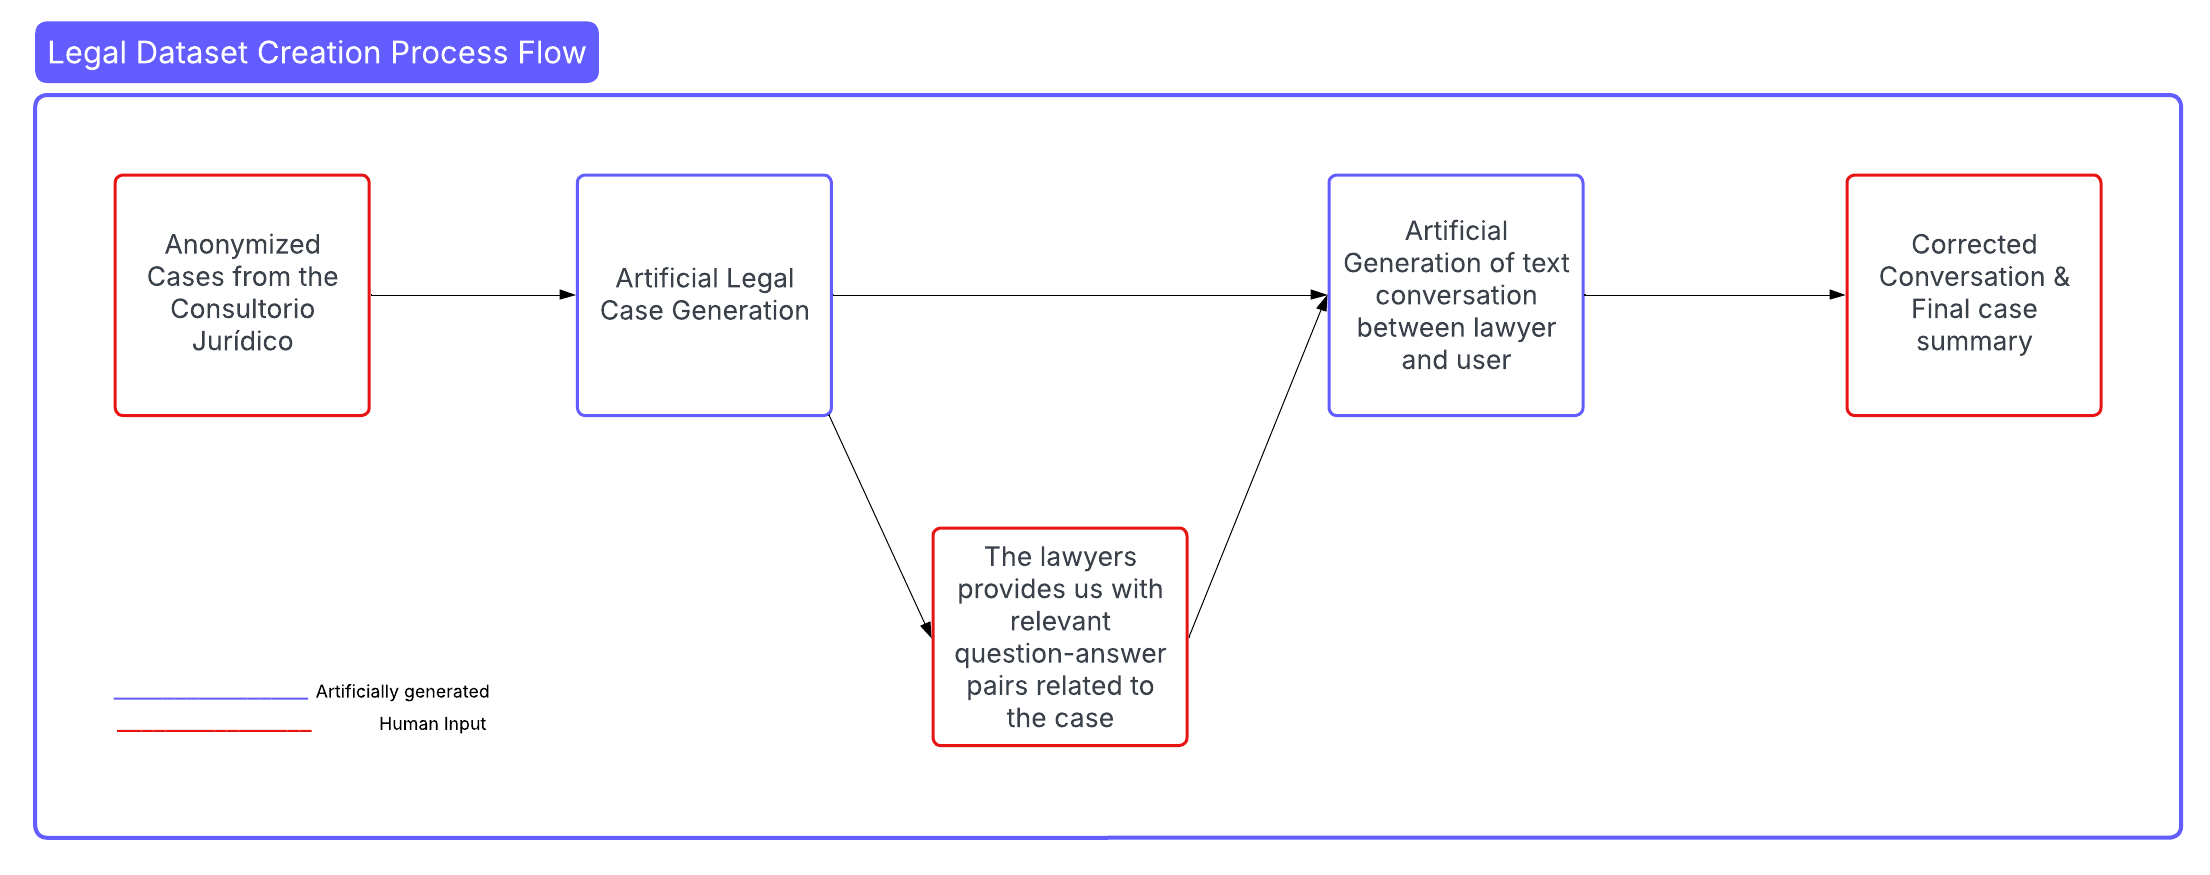
\includegraphics[width=0.7\textwidth]{figures/Legal_dataset.png}
    \caption{Legal Dataset Creation}
    \label{fig:legal_data}
\end{figure}

These phases are Synthetic Case Generation, Expert-Guided Refinement, Conversation simulation and Legal Strategy Development.

\subsection{Base Case Preparation}
The initial phase focused on establishing a foundation of real cases while ensuring privacy of the parties involved:
\begin{itemize}
    \item Initialized with 23 anonymized gender-based case summaries from the Consultorio Jurídico
    \item Categorized cases into primary themes including:
    \begin{itemize}
        \item Violencia Basada en Género
        \item Derechos Sexuales y Reproductivo
        \item Violencia Económica
        \item Violencia Sexual
        \item Violencia en el Ámbito Familiar
        \item Violencia en el Ámbito Laboral
        \item Violencia Institucional
        \item Interseccionalidad
        \item Violencia Pública
        \item Violencia Familiar
    \end{itemize}
\end{itemize}

\subsection{Synthetic Case Generation}
For each base case, we employed GPT-4 with a prompt that included the case category, legal context, 
and example templates from similar cases (see Appendix~\ref{app:prompts}, Section~\ref{sec:content-gen-prompts}, 
Subsection~\ref{subsec:case-gen-prompt}). 
In order to balance consistency and variation within the generated cases, we set the temperature parameter to 0.3. This value was determined empirically, as it maintained variation in cases without making up unrealistic details. This approach enabled us to create a set of synthetic cases that maintained the most characteristics of real legal scenarios while providing sufficient variation for evaluation.

\subsection{Expert-Guided Refinement}
A team of 5 law students and 6 attorneys reviewed the synthetic cases. The review process included case completeness verification, 
development of question-answer pairs, and structural edits. Through this process, legal experts identified and 
added relevant case details that might have been overlooked by the LLM during the generation.

\subsection{Conversation Simulation}
The conversation simulation process transformed the synthetic cases into legal consultations. For each case, 
we used a prompt template that included the case facts, recommended questions, and expected answers
(see Appendix~\ref{app:prompts}, Section~\ref{sec:content-gen-prompts}, 
Subsection~\ref{subsec:legal-consult-prompt}). 
The process can be represented as:

\begin{equation}
    C_{final} = \text{LLM}(P_2(\text{LLM}(P_1(C_{base})))
\end{equation}

where:
\begin{itemize}
    \item $C_{base}$ represents the synthetic case with its facts, questions, and expected answers
    \item $P_1$ is the initial prompt template that structures the conversation
    \item $P_2$ is the refined prompt that incorporates expert feedback
\end{itemize}

The LLM was configured to simulate a legal expert conducting an initial consultation, with the following constraints:
\begin{itemize}
    \item The lawyer starts with no prior knowledge of the case
    \item Questions must be asked to gather all necessary information
    \item The conversation must maintain a professional yet empathetic tone
    \item Legal details must be explained in accessible terms
\end{itemize}

\subsection{Legal Strategy Development}
The evaluation process used the Chatbot's output to generate legal cases. For each conversation, the system produced a legal case 
enriched with relevant legislation through RAG. Legal experts then created their own case summaries based on the same conversations. 
We used BERTScore to measure the similarity between the chatbot-generated cases and the expert-written summaries, 
providing a quantitative measure of the system's ability to produce outputs that are semantically similar to what a legal expert would write.

\subsection{Final Dataset Composition}
The dataset development process was sequential, with each phase building upon the previous one. This resulted in 62 complete cases, each containing:
\begin{itemize}
    \item A synthetic case (Figure~\ref{fig:Artificial_case_summary})
    \item A simulated legal conversation (Figure~\ref{fig:corrected_conversation})
    \item Chatbot-generated legal strategy/summary
    \item An expert-written legal strategy/summary (Figure~\ref{fig:output_summary})
\end{itemize}

The pipeline's sequential nature provided consistency across all cases while allowing for iterative refinement at each stage. 
The synthetic case generation provided a controlled starting point, while the expert-guided refinement added legal context. 
The conversation simulation created simulated interactions, and the final legal strategy development enabled direct comparison 
between the chatbot's output and expert analysis. This structure allows for both qualitative assessment of the chatbot's performance 
and quantitative evaluation through BERTScore metrics.

\begin{figure}[htbp]
    \centering
    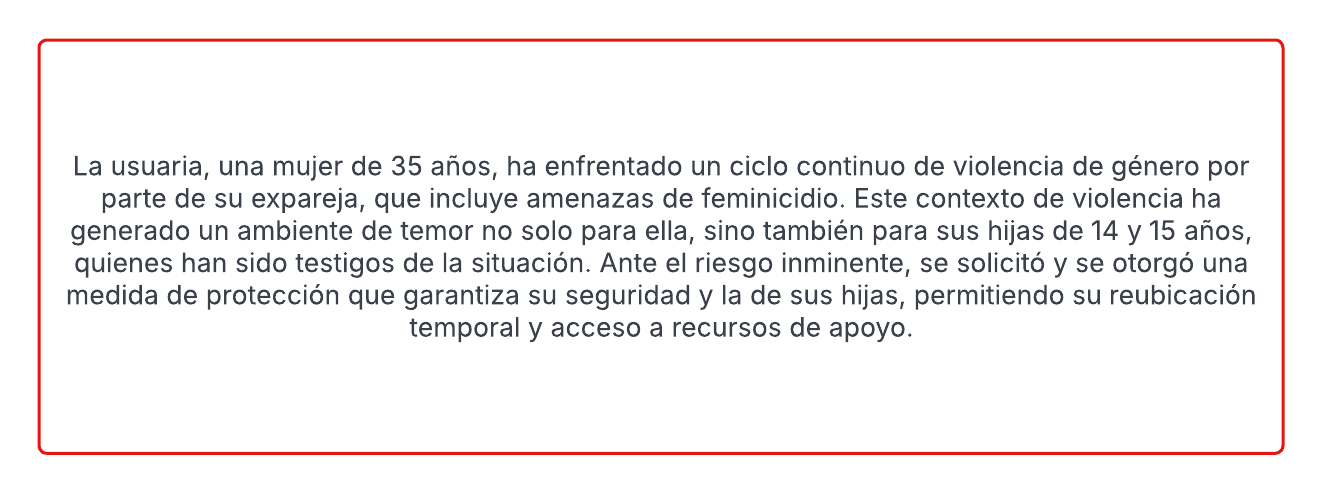
\includegraphics[width=0.7\textwidth]{figures/Artificial_case_summary.png}
    \caption{Example of Artifical Case}
    \label{fig:Artificial_case_summary}
\end{figure}

\begin{figure}[htbp]
    \centering
    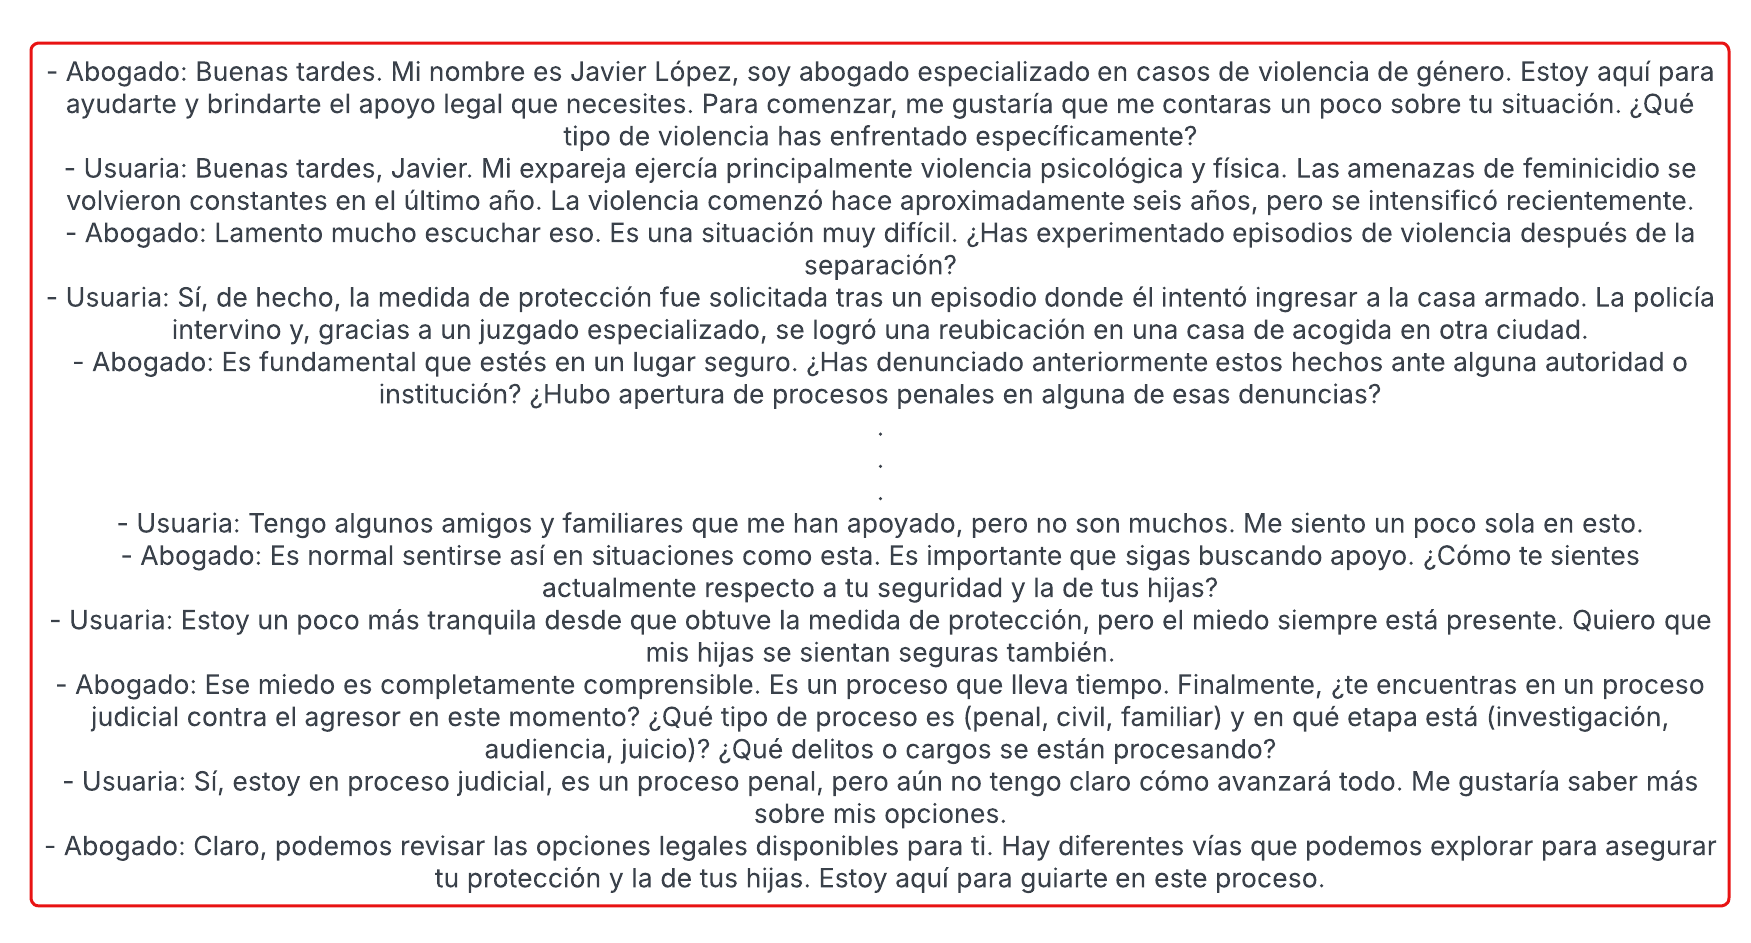
\includegraphics[width=0.7\textwidth]{figures/corrected_conversation.png}
    \caption{Corrected conversation}
    \label{fig:corrected_conversation}
\end{figure}

\begin{figure}[htbp]
    \centering
    
\includegraphics[width=0.7\textwidth]{figures/output_summary.png}
    \caption{Example of a case summary and legal strategy}
    \label{fig:output_summary}
\end{figure}

\section{Agentic Pipeline Development}
\subsection{System Architecture}
\label{sec:architecture}

Our agentic pipeline employs a three-stage architecture for legal case processing, 
as shown in Figure~\ref{fig:chatbot_architecture}. 
Each component operates sequentially with checks between stages.

\begin{figure}[htbp]
    \centering
    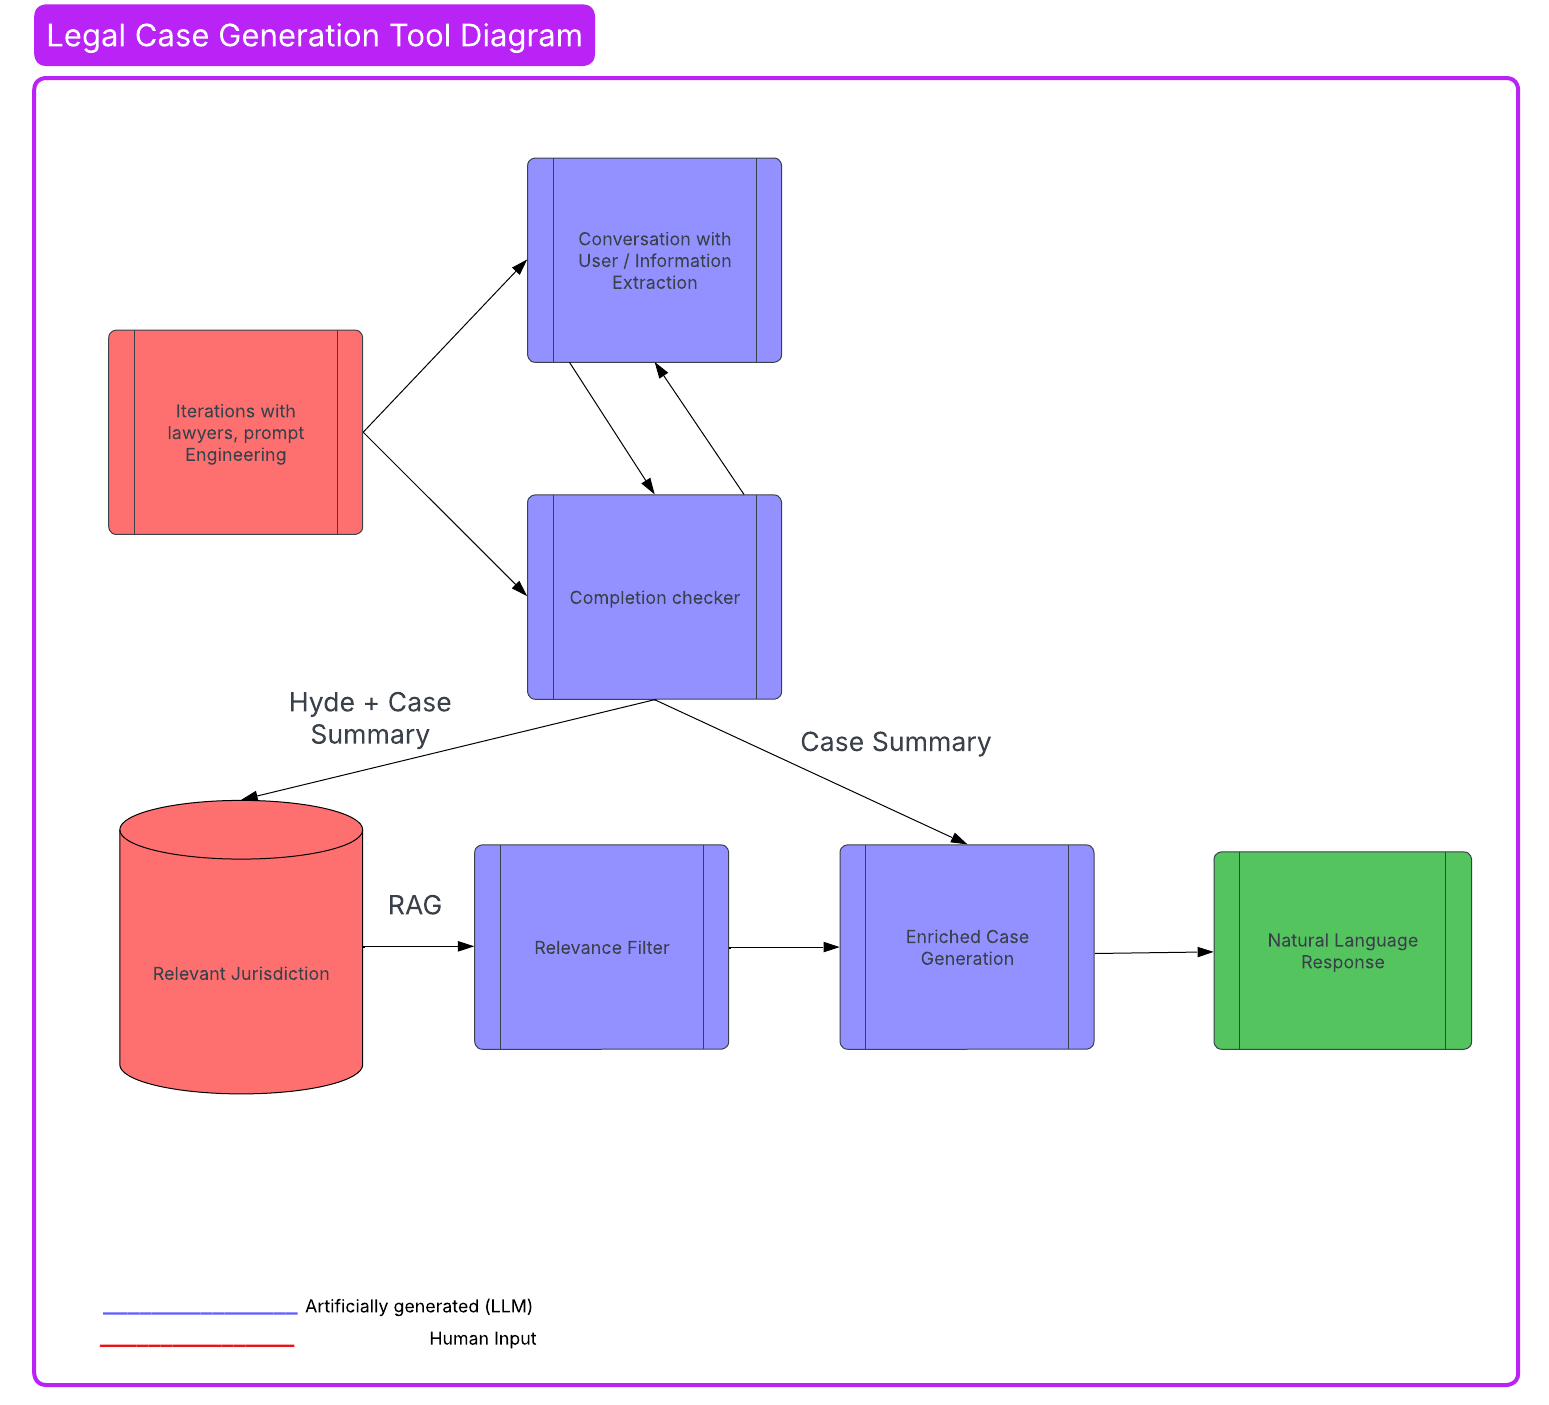
\includegraphics[width=0.7\textwidth]{figures/Chatbot_arch.png}
    \caption{Chatbot Architecture}
    \label{fig:chatbot_architecture}
\end{figure}

\subsection{Information Extraction Module}
The Information Extraction Module is responsible for conducting the initial legal interview with the user. 
Acting as a virtual lawyer, the assistant guides the user through a series of structured questions to collect 
all relevant information about their case, such as the type of violence, the sequence of events, available evidence, 
and the user's objectives. Throughout the conversation, the system manages the state of the interview, keeping track of 
the questions asked, the information gathered, and the user's location within Colombia. The system uses the Legal Interview Prompt 
(see Appendix~\ref{app:prompts}, Section~\ref{sec:legal-interview-prompts}, Subsection~\ref{subsec:legal-interview-prompt}) 
to establish the conversational flow. Due to OpenAI's content safety filters, 
we also preprocess input to handle sensitive content appropriately; this was a particularly difficult task due to the nature 
of the cases and is explored further later. 
After each exchange, the module checks whether enough information has been collected to proceed 
(using the Completion Checker Prompt in Appendix~\ref{app:prompts}, Section~\ref{sec:legal-interview-prompts}, 
Subsection~\ref{subsec:completion-checker-prompt}), either by reaching a predefined threshold or 
by signals from the user or assistant.
\subsubsection{Sensitive Content Handling}
To ensure that conversations could address sensitive topics without being interrupted by content safety filters, 
we implemented a preprocessing step for user input. This was necessary because OpenAI's content moderation system 
can block or flag messages containing explicit or potentially triggering language, which is common in legal cases 
involving violence or abuse. Through some iterations with legal experts, we identified recurring patterns and terms 
that tended to trigger these filters. The function developed for this purpose uses both a dictionary of direct replacements 
and a set of regular expressions to sanitize sensitive content, including sexual, economic, 
physical, and psychological abuse. This preprocessing allows the conversation to remain fluid and focused on the legal issues, 
even when discussing difficult subjects.

\subsection{Legal Case Generation}
The Legal Case Generation module takes the information collected during the interview and organizes it into a structured legal case summary. 
This process involves filtering the conversation data to extract key details, such as the parties involved, the classification of the case, 
a timeline of events, a list of evidence, and the client's main concerns or requests. The module ensures that all relevant facts are included 
and that the information is presented in a format suitable for legal analysis. This structured summary serves as the input for retrieving 
applicable legal documents and generating tailored legal guidance in the subsequent stages.

\subsection{Legal Strategy Generation}
Once the case summary is complete, the system uses a Retrieval-Augmented Generation (RAG) approach to provide legal guidance. 
First, it generates a hypothetical legal document using the HyDE technique 
(see Appendix~\ref{app:prompts}, Section~\ref{sec:legal-interview-prompts}, Subsection~\ref{subsec:hyde-prompt}), 
based on the details of the user's case. The system then searches a 
FAISS vector database containing over 2,000 Colombian legal documents across multiple jurisdictions, including Departamental, Nacional, and 
General categories.

The document database was preprocessed and segmented, with a total of 2,057 individual segments created from the original legal texts. 
Each document was split based on legal hierarchical markers (such as LEY, CAPÍTULO, ARTÍCULO) and labeled with detailed metadata including 
jurisdiction, document name, and specific legal references. This preprocessing enables granular retrieval and contextual matching of legal 
provisions to user cases.

During the retrieval process, the system filters results according to the user's department 
(using the Departamento Extraction Prompt in Appendix~\ref{app:prompts}, Section~\ref{sec:legal-interview-prompts}, 
Subsection~\ref{subsec:departamento-prompt}), int his way, both national and local laws are considered. 
The retrieved legal texts are then incorporated into the final case summary 
(using the RAG Summarizer Prompt in Appendix~\ref{app:prompts}, Section~\ref{sec:legal-interview-prompts}, 
Subsection~\ref{subsec:rag-summarizer-prompt}).

\section{Application Development}

\subsection{Web Application Interface: Initial Prototype}
\label{sec:web-interface}

As part of our development process, we created an initial prototype using Streamlit to test the core functionalities of our legal 
assistance system. This early implementation in served as a proof-of-concept rather than a user-ready solution, 
running entirely on local machines which limited its shareability and accessibility.

\begin{figure}[htbp]
    \centering
    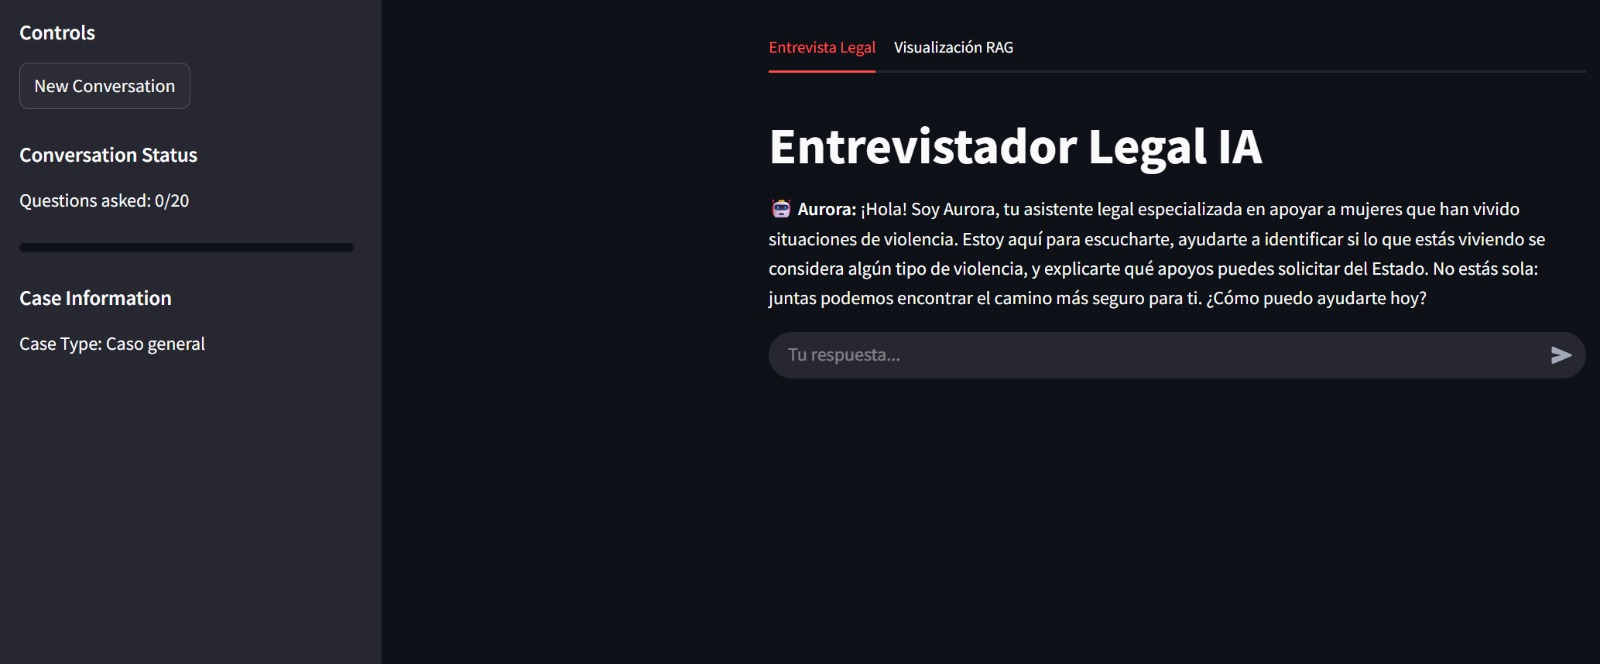
\includegraphics[width=0.7\textwidth]{figures/streamlit.jpeg}
    \caption{Streamlit Interface}
    \label{fig:streamlit}
\end{figure}

\subsubsection{Prototype Interface}
The prototype featured a straightforward interface. 
The Legal Interview section provided a basic chat interface where users could interact with "Aurora". \ref{fig:streamlit}

When a case was completed, the prototype would display a simple success message and the final case summary.

\subsubsection{Technical Limitations}

%This initial prototype faced some technical constraints:
%The application ran exclusively on local development machines, requiring users to have Python and all dependencies installed. 
%This severely limited its shareability and made it impractical for any real-world testing with legal professionals or users.
While deployment was technically possible, it would have significantly limited our customization options. Besides, 
given that the end goal was to create a fully-featured application, developing a proper API architecture
would ultimately provide much greater reliability and flexibility than the Streamlit-based approach.
The interface relied on Streamlit's session state for managing conversation history, which occasionally led to state management 
issues during longer interactions. Message format conversion between the UI and the underlying LangChain components was handled 
through direct manipulation of data structures.

While the prototype implemented the sensitive content preprocessing to avoid content filter issues, 
this solution was not tested. Document rendering was functional but basic, 
with limited formatting options for the legal texts.

\subsubsection{Learning from the Prototype}

Despite its limitations, the initial Streamlit prototype was valuable in revealing insights that would inform later development:
The need for a cloud-based deployment that wouldn't require users to run code locally became evident immediately.

The prototype also demonstrated that while Streamlit was excellent for rapid prototyping, a more robust framework would be needed for a user-ready 
application with better performance and customization options.

This early implementation represented an important step in our development process, allowing us to test functionalities and gather 
feedback that would shape the versions that followed.

\subsection{User Web Application Development}
\label{subsec:web-application}

Following the insights gained from our initial Streamlit prototype, we developed a web application architecture that addressed the limitations of the prototype and enabled broader customization and easier deployment.

%\begin{figure}[htbp]
%    \centering
%    \includegraphics[width=0.8\textwidth]{figures/webapp_architecture.png}
%    \caption{Web Application Architecture}
%    \label{fig:webapp_architecture}
%\end{figure}

\subsubsection{FastAPI Backend Service}

The backend of our production system was implemented using FastAPI, a web framework for building APIs with Python. 
This choice offered many advantages over the Streamlit prototype:
The backend service provided a set of REST endpoints for conversation management, including initializing conversations, sending and receiving messages, 
retrieving case summaries, and accessing RAG documents. This API-centric approach decoupled the Frontend from the underlying AI logic, allowing for multiple client 
applications to connect to the same backend service.

To solve the state management issues encountered in the prototype, we implemented MongoDB integration for conversation persistence. This allowed the system to store 
conversation states, legal contexts, and retrieved documents, enabling long-term storage of user interactions.

The backend handled the complete conversation life-cycle, processing user messages through the legal interview model, 
detecting when cases were completed, triggering the RAG system to retrieve relevant legal documents, and managing the transition 
between conversation and legal summary generation.

We refined the Colombian location detection capabilities to provide more region-specific legal information, implementing detection of Colombian departments in user messages. 
The system also included error handling and logging to diagnose and troubleshoot issues.

\subsubsection{Web Client Implementation}

To make the application accessible to a wide range of users, we developed a lightweight frontend interface:
The frontend was implemented as a static web application using JavaScript and HTML, delivered through a minimal Node.js server. This approach resulted in a design that works across different devices and screen sizes, making the legal assistant accessible from desktop computers, tablets, or mobile phones.

The interface was designed for simplicity and usability, focusing on the conversational interaction with the AI assistant. 
When legal information was retrieved, it was presented along the summary. \ref{fig:Frontend}

The frontend communicated with the backend exclusively through the REST API, allowing for a clean separation of concerns between 
the user interface and the backend processing logic.

\begin{figure}[htbp]
    \centering
    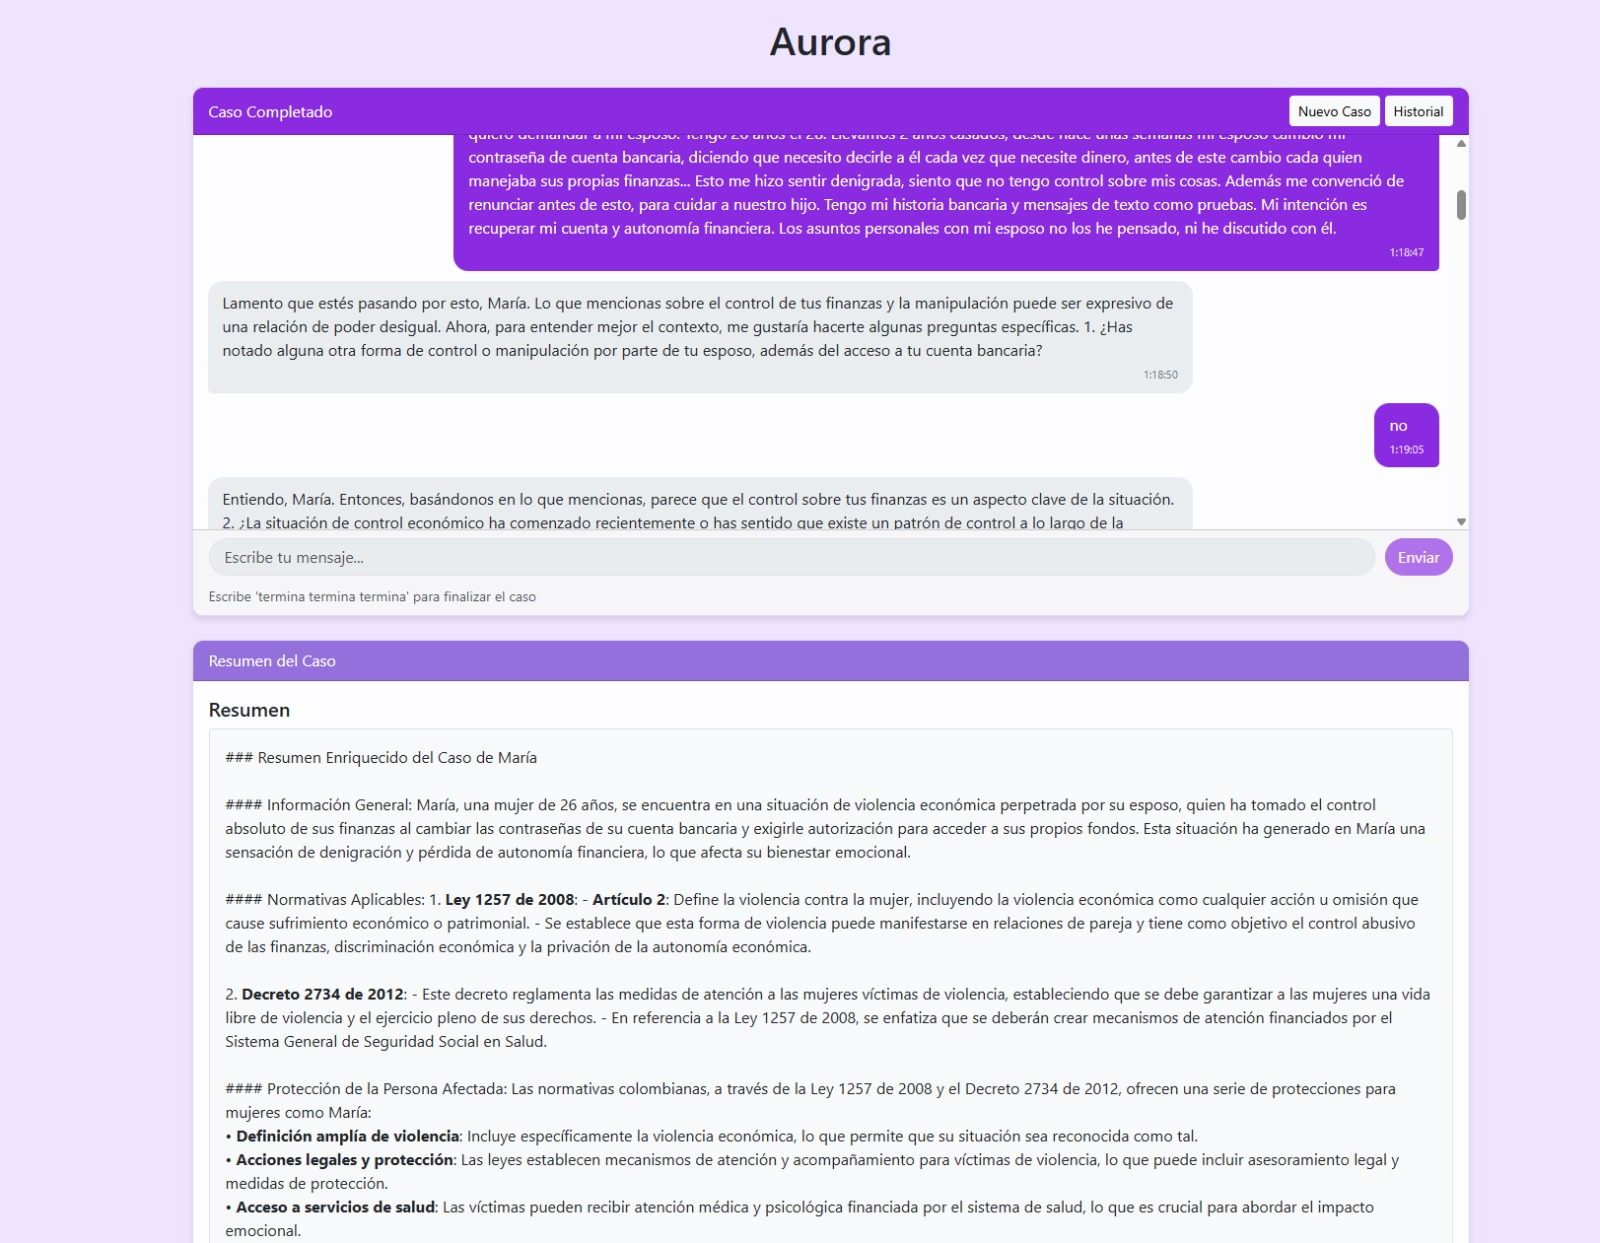
\includegraphics[width=0.8\textwidth]{figures/Frontend.jpeg}
    \caption{Web Application UI}
    \label{fig:Frontend}
\end{figure}

\subsubsection{Containerization and Cloud Deployment}

To facilitate deployment and ensure consistency across environments, the entire application was containerized using Docker:

The containerization process included packaging all required components: the FAISS index for document retrieval, preprocessed legal documents, 
and model code, so that the application had access to all necessary resources regardless of the deployment environment.
For deployment, we developed an automated script that orchestrated the deployment of both backend and frontend components to Google Cloud Run. 

The cloud deployment strategy enabled global accessibility while maintaining reasonable costs, as Cloud Run's serverless architecture only incurred charges when the 
application was actively being used.

\subsection{Initial User Testing}
\label{subsec:user-testing}

To assess the effectiveness of our web application, we conducted limited user testing with a small group of participants including law students, legal professionals, 
and individuals without legal backgrounds. This testing was designed to find the most common issues and improve the system in a very empirical way.

The testing process involved participants engaging with the assistant covering different types of gender-based legal cases as they wished. After each interaction, 
these participants provided feedback on the ease of use, clarity of information, and perceived helpfulness of the legal guidance provided.

This feedback was valuable in understanding both the strengths and limitations of our approach. The positive reception of the conversational interface validated our design 
decisions, while the critiques revealed issues requiring attention.

A significant problem identified during testing was that the RAG system was not behaving optimally. It frequently recommended legal documents that were not applicable to the 
user's specific situation, particularly when regional or departmental legislation was involved. This discovery led us to develop the departamento extraction feature, 
which enabled the system to specifically ask users about their location in Colombia and then filter out non-applicable legislation. This targeted approach  
improved the relevance of the document retrieval process, as users wouldn't receive guidance that was not applicable to them given their geographic location.

Additionally, the testing highlighted the importance of the assistant's tone and communication style. Lawyers from the Consultorio Jurídico emphasized that legal assistants 
in gender-based cases must be especially empathetic and supportive, as clients are often in vulnerable situations. Based on this input, we significantly refined the system's 
prompts to ensure a friendly, supportive, and non-judgmental approach while still maintaining professional boundaries and accuracy.

\subsection{Iterative Prompt Engineering}
\label{subsec:prompt-engineering}

Throughout the development process, an important aspect of our methodology was the iterative refinement of system prompts in close collaboration with legal professionals. 
The prompts detailed in Appendix~\ref{app:prompts} were not static instructions created at the outset of the project, but rather evolved significantly through  
feedback cycles with practicing lawyers and legal scholars. 

The information gathering process itself was structured based on direct input from lawyers at the Consultorio Jurídico. They provided detailed guidance on the specific types of 
information needed to properly assess and address gender-based legal cases in Colombia. This included the appropriate questions, critical data points to collect 
(such as relationship to the aggressor, types of violence experienced, and available evidence), and how to approach sensitive topics in a trauma-informed manner.

This collaborative prompt engineering process involved review sessions where legal experts would interact with the tool, check its legal summaries, and produced document 
retrievals. Their feedback guided substantial revisions to prompt wording, structure, and content focus.

%The iterative prompt engineering process highlights the importance of interdisciplinary collaboration in developing AI systems for specialized domains. 
%While large language models provide powerful capabilities, harnessing these capabilities for domain-specific applications requires ongoing dialogue between 
%technical developers and subject matter experts. The final prompts represent a synthesis of computational and legal knowledge.
\chapter{Evaluation}
\section{Evaluation Framework}
The evaluation of the agentic pipeline was done in collaboration with legal students and experts
\begin{table}[h]
    \centering
    \caption{Criteria Framework for Human Evaluation of Legal AI System}
    \begin{tabular}{p{3cm}p{12cm}}
    \hline
    \textbf{Criterion} & \textbf{Description} \\
    \hline
    Legal Accuracy & This metric assesses whether the legal information provided in the system's output is factually correct, consistent with Colombian law, and properly interprets relevant statutes, regulations, and precedents applicable to gender-based cases. \\
    \hline
    Completeness & This metric evaluates whether the system extracts all necessary information during the conversational phase to form a comprehensive understanding of the case, without missing critical details that would affect the legal strategy. \\
    \hline
    Relevance & This metric measures whether the legal strategies and guidance generated by the system are directly applicable to the specific circumstances of the case, address the core legal issues at hand, and provide actionable next steps tailored to the user's situation. \\
    \hline
    Clarity & This metric assesses whether the legal guidance is communicated in language that is accessible to users with limited legal literacy, avoids unnecessary jargon, explains technical concepts when needed, and presents information in a logical, easy-to-follow structure. \\
    \hline
    Conversational Appropriateness & This metric evaluates the system's ability to conduct sensitive conversations about gender-based legal issues, including appropriate phrasing of questions, recognition of emotional contexts, and maintenance of a supportive, non-judgmental tone throughout the interaction. \\
    \hline
    Procedural Correctness & This metric examines whether the system accurately identifies and explains the proper legal procedures, timelines, documentation requirements, and institutional pathways relevant to the user's case within the Colombian justice system. \\
    \hline
    Legal Utility & This metric evaluates the practical value of the system's output for users navigating gender-based legal issues, including actionability of advice, prioritization of critical information, and potential to improve user outcomes in the legal process. \\
    \hline
    \end{tabular}
\end{table}

\subsection{Evaluation Methodology}
The evaluation of our agentic pipeline for gender-based legal cases 
incorporates both automated metrics and human assessment. For automated 
evaluation, we employ two complementary approaches:
\subsubsection{BERTScore for Semantic Similarity}
We utilize BERTScore~\cite{zhang2020bertscoreevaluatingtextgeneration} to measure the semantic similarity between system-generated legal strategies and reference strategies prepared by legal experts. Unlike surface-level metrics such as BLEU or ROUGE, 
BERTScore leverages contextual embeddings to capture deeper semantic 
correspondence, making it particularly suitable for evaluating legal 
content where precise meaning is critical. For each test case, we compute 
precision, recall, and F1 scores using:
\begin{equation}
P_{BERT} = \frac{1}{|x|}\sum_{x_i \in x}\max_{y_j \in y}\cos(e(x_i), e(y_j))
\end{equation}
\begin{equation}
R_{BERT} = \frac{1}{|y|}\sum_{y_j \in y}\max_{x_i \in x}\cos(e(x_i), e(y_j))
\end{equation}
\begin{equation}
F_{BERT} = 2\frac{P_{BERT} \cdot R_{BERT}}{P_{BERT} + R_{BERT}}
\end{equation}
where $e(\cdot)$ represents contextualized embeddings from a pre-trained language model fine-tuned on Colombian legal texts.

\subsubsection{LLM-based Relevance Classification for RAG}
To evaluate the effectiveness of our RAG component, we implement a 
prompt-engineering approach for relevance classification~\cite{es2023ragasautomatedevaluationretrieval}. 
For each retrieved document chunk, we design a systematic prompt 
that instructs the LLM to assess relevance with a binary classification:

\begin{verbatim}
Given the legal case context: [CASE DESCRIPTION]
Evaluate the following document chunk for relevance:
[RETRIEVED DOCUMENT CHUNK]

Respond ONLY with 'RELEVANT' or 'NOT RELEVANT' 
based on whether this chunk directly supports 
resolving the legal issue described.
\end{verbatim}

This method leverages the zero-shot capabilities of large language 
models to perform binary classification without requiring extensive 
fine-tuning. We apply this approach across a diverse set of gender-based 
legal cases, collecting relevance assessments for multiple retrieved 
document chunks.

The evaluation metrics are computed as follows:
\begin{equation}
Precision = \frac{|\text{Retrieved Relevant Documents}|}{|\text{All Retrieved Documents}|}
\end{equation}

\begin{equation}
Recall = \frac{|\text{Retrieved Relevant Documents}|}{|\text{All Relevant Documents}|}
\end{equation}

We acknowledge the potential limitations of this approach, including 
prompt sensitivity and the need for careful prompt design. To mitigate 
these concerns we conduct human validation to cross-check the LLM's relevance assessments~\cite{es2023ragasautomatedevaluationretrieval}.

The primary objective is to quantify the retrieval component's 
effectiveness by analyzing the proportion of contextually relevant 
documents retrieved for each legal case scenario. This approach provides 
an automated method for assessing RAG performance, complementing our 
human evaluation framework.

\section{Evaluation Methodology for Agentic Components}
Our evaluation strategy recognizes the distinctive challenges posed by 
each agent within the legal guidance pipeline. The methodology balances 
quantitative precision with qualitative insight, acknowledging the nuanced 
nature of legal communication.

The information extraction agent, responsible for conversationally 
gathering case details, will be assessed through a mixed-methods approach. 
Quantitative metrics will measure the completeness and accuracy of 
information gathered, tracking the agent's ability to systematically 
elicit critical legal context. Simultaneously, leveraging the previously 
developed database, we evaluate the model’s legal strategy generation by 
measuring its proximity to the ground truth using BERTScore, assessing 
its performance in this specific task.

For the retrieval-augmented generation (RAG) component, our evaluation 
centers on semantic relevance and source credibility. The previously 
discussed BERTScore and LLM-based relevance classification will provide 
computational metrics assessing how precisely retrieved legal documents 
align with the specific case context. These automated evaluations will 
be complemented by expert reviews, where legal professionals assess the 
substantive accuracy and jurisdictional appropriateness of the retrieved 
sources.

The communication agent demands a more nuanced evaluation framework. 
Beyond traditional linguistic metrics, we will employ user experience 
surveys and expert assessments to gauge the agent's ability to translate 
complex legal strategies into accessible, actionable guidance. The goal 
is to measure not just linguistic clarity, but the agent's capacity to 
demystify legal processes for individuals with varying levels of legal 
literacy.


By integrating computational metrics with human expertise, our evaluation 
methodology seeks to move beyond traditional performance assessments. 
We aim to develop a holistic understanding of how AI can effectively 
support legal empowerment, particularly for marginalized communities 
navigating complex gender-based legal challenges.

\section{Legal Specific questions Questions}
Legal Accuracy:
¿En qué medida la información legal proporcionada por el sistema es precisa, actualizada y correctamente contextualizada dentro del marco jurídico colombiano sobre asuntos de género?

Completeness:
¿Hasta qué punto el sistema solicita y extrae toda la información relevante y necesaria durante la fase conversacional, sin omitir detalles críticos que podrían afectar la estrategia legal?

Relevance:
¿En qué grado las estrategias legales y orientaciones generadas por el sistema responden directamente a las circunstancias específicas del caso y proporcionan pasos accionables adaptados a la situación particular?

Clarity:
¿Con qué eficacia el sistema comunica información legal compleja en un lenguaje accesible, evitando jerga innecesaria y explicando conceptos técnicos de manera que resulten comprensibles para usuarios sin formación jurídica?

Conversational Appropriateness:
¿En qué medida el sistema maneja conversaciones sobre temas sensibles relacionados con género, demostrando empatía, utilizando un lenguaje apropiado y manteniendo un tono de apoyo y no crítico durante toda la interacción?

Procedural Correctness:
¿Con qué precisión el sistema identifica y explica los procedimientos legales, plazos, requisitos documentales y vías institucionales específicas aplicables al caso dentro del sistema judicial colombiano?

Legal Utility:
¿En qué grado los consejos y recomendaciones proporcionados por el sistema tienen valor práctico para mejorar los resultados del usuario en el proceso legal, incluyendo la priorización efectiva de información crítica y pasos accionables?

for each question the system will be evaluated with a score from 1 to 5.



Moreover we will use the CUQ questionaire for actual layover people
when finishing the process in order to get feedback on the 
bot's more general performance. [citation!!!!]
\chapter{Conclusion and Future Work}
\subsection{Future Work and Limitations}
The lack of data may have been one of the biggest limitations encountered when approaching the
problem presented.
%\include{CHAPTER_FILE_NAME}


%Adding appendices if needed
\appendix
% $Id: appendix-a. $
% !TEX root = main.tex

\chapter{System Prompts}
\label{app:prompts}

This appendix contains the prompts used in this thesis project, organized by module.

\section{Legal Interview System Prompts}
\label{sec:legal-interview-prompts}

\subsection{Legal Interview Prompt}
\label{subsec:legal-interview-prompt}
\begin{lstlisting}[style=prompt]
Tu Nombre es Aurora,
Eres una abogada experta en derecho Colombiano, especialista en genero.
Debes iniciar la conversación presentándote y pidiendo al cliente que describa brevemente su situación.
Luego, Realiza preguntas claras y específicas para recopilar información sobre el caso legal de la cliente.


Debes cubrir estos aspectos:
    0.  Nombre de la persona entrevistada, ciudad de ressidencia si se siente cómoda con ello.
    1.  Identificación completa de las partes involucradas (edad, relación con el agresor: puede ser pareja, expareja, familiar, conocido o incluso desconocido. situación de desigualdad o subordinación: ¿Existe una relación de poder o control?
    2.  Identificar el tipo de violencia aplica a la situación: (1.Física: Golpes, empujones, quemaduras, agresiones con objetos, etc. (2. Psicológica o emocional: Insultos, humillaciones, amenazas, manipulación, aislamiento, etc. (3. Sexual: Cualquier acto sexual no consentido, acoso, abuso, violación. (4. Económica o patrimonial: Control del dinero, despojo de bienes, prohibición de trabajar. (5. Institucional: Negligencia o trato discriminatorio por parte de autoridades o personal público. (6 Digital: Acoso, amenazas o difusión de contenido íntimo sin consentimiento en medios digitales.)
    3.  Cronología detallada de los hechos: cuándo comenzaron, frecuencia, eventos importantes. Elementos contextuales del delito
    •   Frecuencia y patrón de violencia: ¿Es un hecho aislado o repetido?
    •   Escalada: ¿La violencia ha ido aumentando en intensidad?
    •   Aislamiento o control: ¿La víctima está siendo vigilada, controlada o alejada de su red de apoyo?
    •   Dependencia económica o emocional: ¿Hay factores que dificultan que la víctima salga de la situación?
    4. Afectación a derechos
    •   Integridad física o emocional
    •   Libertad sexual o reproductiva
    •   Libertad de tránsito o decisión
    •   Acceso a la justicia


    5.⁠ ⁠Documentación o pruebas mencionadas (denuncias, partes médicos, testigos, mensajes, fotos, etc.). Testimonios consistentes
    •   Documentación médica o psicológica
    •   Mensajes, correos, grabaciones, fotografías
    •   Denuncias anteriores o medidas de protección
    •   Testigos (familiares, vecinos, personal médico, etc.)
    6.  Pretensiones u objetivos de la persona entrevistada (qué busca: protección, denuncia, asesoría, custodia, etc.).


Consejos para mejorar tu enfoque:
- Evita preguntas excesivamente personales o gráficas.
- Utiliza lenguaje respetuoso y profesional (Haz uso de "tuteo", nunca te refieras al cliente como "usted" ni uses el adjetivo posesivo "su". únicamente "tu").
- Mantén un enfoque firme en recopilar la información legalmente relevante.
- No Siempre debes hacer preguntas, lee el ambiente y considera cuidadosamente si es pertinente hacer una pregunta tomar otra acción.
- Pregunta amablemente en qué departamento de Colombia se encuentra la persona, ya que esto te ayudará a proporcionar información legal más específica y relevante a su ubicación.


IMPORTANTE:
1. Tu primera pregunta debe ser empática y abierta, enfocada en comprender la situación.
2. Para establecer interacción, incluye siempre una pregunta a la persona pero limita a una pregunta por turno.
3. Cuando consideres que tienes suficiente información para comprender el caso, puedes indicar que el resumen está listo.
4. Antes de finalizar, confirma si la persona está en algún departamento específico de Colombia, si aún no lo ha mencionado.


IMPORTANTE: Al tratar temas sensibles, utiliza terminología legal profesional y evita lenguaje explícito.
Para casos relacionados con explotación laboral, acoso, o engaño,
enfoca la discusión en los aspectos legales como: consentimiento informado, incumplimiento contractual,
falsas representaciones, coacción, o violación de derechos laborales.


Lleva un registro de cuántas preguntas has hecho en la conversación. Cuando hayas hecho
20 preguntas, finaliza la entrevista indicando que has recopilado suficiente información.
- Si el usuario esta bajo peligro, DEBES marcar el caso como incompleto y finalizar, incluso si falta alguna
información menor, señalando que número de emergencia se debe llamar.
\end{lstlisting}

\subsection{Completion Checker Prompt}
\label{subsec:completion-checker-prompt}
\begin{lstlisting}[style=prompt]
Eres un asistente legal especializado en verificar la completitud de la información de casos legales.
Tu tarea es analizar la conversación y determinar si se ha recopilado toda la información necesaria.


A continuación verás la transcripción de una entrevista legal realizada a una mujer que busca orientación por una situación de violencia. Tu tarea es revisar cuidadosamente si la información recopilada incluye los siguientes elementos clave:
    1.  Identificación completa de las partes involucradas (edad, relación con el agresor: puede ser pareja, expareja, familiar, conocido o incluso desconocido. situación de desigualdad o subordinación: ¿Existe una relación de poder o control?
    2.  Identificar el tipo de violencia aplica a la situación: (1.Física: Golpes, empujones, quemaduras, agresiones con objetos, etc. (2. Psicológica o emocional: Insultos, humillaciones, amenazas, manipulación, aislamiento, etc. (3. Sexual: Cualquier acto sexual no consentido, acoso, abuso, violación. (4. Económica o patrimonial: Control del dinero, despojo de bienes, prohibición de trabajar. (5. Institucional: Negligencia o trato discriminatorio por parte de autoridades o personal público. (6 Digital: Acoso, amenazas o difusión de contenido íntimo sin consentimiento en medios digitales.)
    3.  Cronología detallada de los hechos: cuándo comenzaron, frecuencia, eventos importantes. Elementos contextuales del delito
    •   Frecuencia y patrón de violencia: ¿Es un hecho aislado o repetido?
    •   Escalada: ¿La violencia ha ido aumentando en intensidad?
    •   Aislamiento o control: ¿La víctima está siendo vigilada, controlada o alejada de su red de apoyo?
    •   Dependencia económica o emocional: ¿Hay factores que dificultan que la víctima salga de la situación?
    4. Afectación a derechos
    •   Integridad física o emocional
    •   Libertad sexual o reproductiva
    •   Libertad de tránsito o decisión
    •   Acceso a la justicia


    5.⁠ ⁠Documentación o pruebas mencionadas (denuncias, partes médicos, testigos, mensajes, fotos, etc.). Testimonios consistentes
    •   Documentación médica o psicológica
    •   Mensajes, correos, grabaciones, fotografías
    •   Denuncias anteriores o medidas de protección
    •   Testigos (familiares, vecinos, personal médico, etc.)
    6.  Pretensiones u objetivos de la persona entrevistada (qué busca: protección, denuncia, asesoría, custodia, etc.).


si el usuario escribe ´´´termina termina termina´´´ DEBES terminar el proceso.
si alguno de los dos se despide terminar el proceso.


IMPORTANTE: 
- Si han ocurrido más de 20 intercambios en la conversación O el agente entrevistador ha indicado
que ha recopilado suficiente información, DEBES marcar el caso como completo, incluso si falta alguna
información menor. 
- Si el usuario esta bajo peligro, DEBES marcar el caso como incompleto y finalizar, incluso si falta alguna
información menor, señalando que número de emergencia se debe llamar.
- Recordar, no siempre debes hacer una pregunta por turno, si el usuario esta hablando de algo que no tiene que ver con el caso, puedes hacer una pregunta o no.

Primero que nada, incluye en el resumen el tipo de caso (pueden ser varios) (Violencia Basada en Género, Derechos Sexuales y Reproductivos, Violencia Económica,
Violencia Sexual, Violencia en el Ámbito Familiar, Violencia en el Ámbito Laboral,
Violencia Institucional, Interseccionalidad, Violencia Pública o Violencia Familiar)
Intenta incluir toda la información necesaria dentro del resumen.


Debes responder EXCLUSIVAMENTE con un JSON válido que contenga:
{
    "is_complete": boolean,
    "missing_info": [lista de información faltante],
    "summary": "resumen estructurado si is_complete es true O que falta si is_complete es false"
}
\end{lstlisting}

\subsection{RAG Summarizer Prompt}
\label{subsec:rag-summarizer-prompt}
\begin{lstlisting}[style=prompt]
Eres un especialista legal colombiano en casos de género, tu tarea es generar un resumen legal enriquecido.

A continuación verás la conversación de una entrevista legal y la información básica del caso.
Además, recibirás fragmentos de normativas colombianas que son relevantes para este caso.

Información del caso:
{case_summary}

Tipo de caso: {case_type}

Normativas relevantes:
{legal_context}

Si el caso no contiene información relevante, DEBES responder con "No hay información relevante para este caso".

Tu tarea es:
1. Crear un resumen enriquecido del caso que incorpore las normativas aplicables
2. Identificar los artículos específicos de las leyes colombianas que aplican
3. Explicar cómo estas normativas protegen a la persona afectada
4. Sugerir las posibles vías legales disponibles según la legislación colombiana

Responde con un resumen estructurado que sea útil para un profesional legal que va a tomar este caso.
\end{lstlisting}

\subsection{Hypothetical Document Prompt}
\label{subsec:hyde-prompt}
\begin{lstlisting}[style=prompt]
Eres un experto en derecho colombiano especializado en casos de género.
                        
Basado en el siguiente resumen de caso y tipo de caso, genera un documento legal hipotético que contenga las normativas, 
leyes, artículos y jurisprudencia colombiana que serían relevantes para este caso.
                        
Resumen del caso: {case_summary}
Tipo de caso: {case_type}

Si el caso no contiene información relevante, DEBES responder con "No hay información relevante para este caso".   

Genera un documento legal detallado que incluya:
1. Referencias específicas a leyes colombianas aplicables
2. Artículos específicos de esas leyes
3. Jurisprudencia relevante
4. Normativas departamentales o municipales si aplican
                        
Escribe como si fuera un documento legal real que podría ser utilizado como referencia para este caso.
\end{lstlisting}

\subsection{Relevance Filter Prompt}
\label{subsec:relevance-filter-prompt}
\begin{lstlisting}[style=prompt]
Eres un abogado experto en derecho colombiano especializado en casos de género.
                        
Tu tarea es determinar si el siguiente fragmento legal es RELEVANTE o NO RELEVANTE 
para el caso descrito y el documento hipotético generado.
sí el documento hipotético no contiene información relevante, DEBES responder con "NO RELEVANTE".
                        
Resumen del caso: {case_summary}
Tipo de caso: {case_type}
                        
Documento legal hipotético generado:
{hypothetical_document}
                        
Fragmento legal a evaluar:
{document_content}
                        
Evalúa cuidadosamente si este fragmento es relevante para este caso específico.
                        
Responde ÚNICAMENTE con una de estas dos opciones: "RELEVANTE" o "NO RELEVANTE".
\end{lstlisting}

\subsection{Departamento Extraction Prompt}
\label{subsec:departamento-prompt}
\begin{lstlisting}[style=prompt]
De este mensaje de usuario, extrae el departamento de Colombia mencionado, si existe:
"{text}"

Respuesta: Si existe un departamento mencionado, devuelve solo el nombre del departamento.
Si no existe un departamento mencionado, responde "No departamento".
\end{lstlisting}

\section{Content Generation Prompts}
\label{sec:content-gen-prompts}

\subsection{Case Generator Prompt}
\label{subsec:case-gen-prompt}
\begin{lstlisting}[style=prompt]
Por favor, genera un caso legal formal y profesional de tipo "{caso_tipo}". 
El caso debe ser apropiado para un contexto legal y académico.

Utiliza el siguiente formato, manteniendo un tono profesional y evitando detalles explícitos:

1. **Resumen de los hechos o relato de la víctima:**
Genera un resumen profesional y respetuoso basado en: {ejemplo_hechos}

2. **Resumen estrategia jurídica:**
Desarrolla una estrategia legal basada en: {ejemplo_estrategia}

3. **Descripción de la buena práctica:**
Describe acciones profesionales implementadas considerando: {ejemplo_practica}

4. **Principales logros:**
Menciona resultados positivos inspirados en: {ejemplo_logros}

5. **Principales dificultades:**
Describe desafíos profesionales basados en: {ejemplo_dificultades}

6. **Recomendaciones:**
Sugiere mejoras considerando: {ejemplo_recomendaciones}

7. **Lecciones aprendidas:**
Comparte aprendizajes profesionales según: {ejemplo_lecciones}

8. **Códigos éticos:**
Lista principios éticos relevantes tomando como referencia: {ejemplo_codigos}
\end{lstlisting}

\subsection{Legal Consultation Simulator Prompt}
\label{subsec:legal-consult-prompt}
\begin{lstlisting}[style=prompt]
Genera una conversación simulada entre un experto legal y un cliente, basándote en los siguientes detalles:

Contexto de los hechos:
{hechos}

Preguntas al cliente:
{preguntas}

Respuestas esperadas:
{respuestas_esperadas}

Instrucciones para la conversación:
1. La conversación debe ser realista y profesional
2. El abogado debe hacer preguntas aclaratorias cuando sea necesario
3. Incluye detalles legales relevantes
4. La conversación debe cubrir todas las preguntas y proporcionar contexto legal
5. Mantén un tono empático pero profesional
6. Estructura la conversación como un diálogo de entrevista legal
7. El usuario no tienen ningun tipo de conocimiento legal

Formato de salida:
- Abogado: [Intervención del abogado]
- Usuaria: [Respuesta del cliente]

Comienza la conversación con una introducción profesional del abogado. se debe tener en cuenta que el abogado no cuenta con ningun tipo de información sobre el caso, 
por lo que esta información debe llegar a través de la conversación.
Únicamente proporciona la conversación, nada más.
\end{lstlisting}

\endinput



\backmatter
\bibliography{bib/local,bib/writing}

\printindex
\addcontentsline{toc}{chapter}{List of Terms}
\printindex[symbols]
\include{acronym}
\end{document}

\endinput

